\chapter{Exploring the Data}
\label{ChapterIIIb}
\section{Introduction}

Statistician John Tukey is a strong advocate for exploratory data analysis (EDA).  Collectively, EDA is a series of graphical and quantitative techniques used to explore novel data in order to examine its data structure, and thus generate insights that can be used as a springboard for hypothesis and model generation \citep{tukey77,Hoaglin1982}.  

This chapter performs EDA on the data at various ground scales (country, state, core-based statistical area (CBSA), county and point) using a variety of techniques such as simple counts to more elaborate techniques such as Ripley's K and the gravity model of trade. 

\nomenclature{EDA}{Exploratory Data Analysis}
\section{Count and Percentage by Region}
\begin{figure}[h]
	\centering
	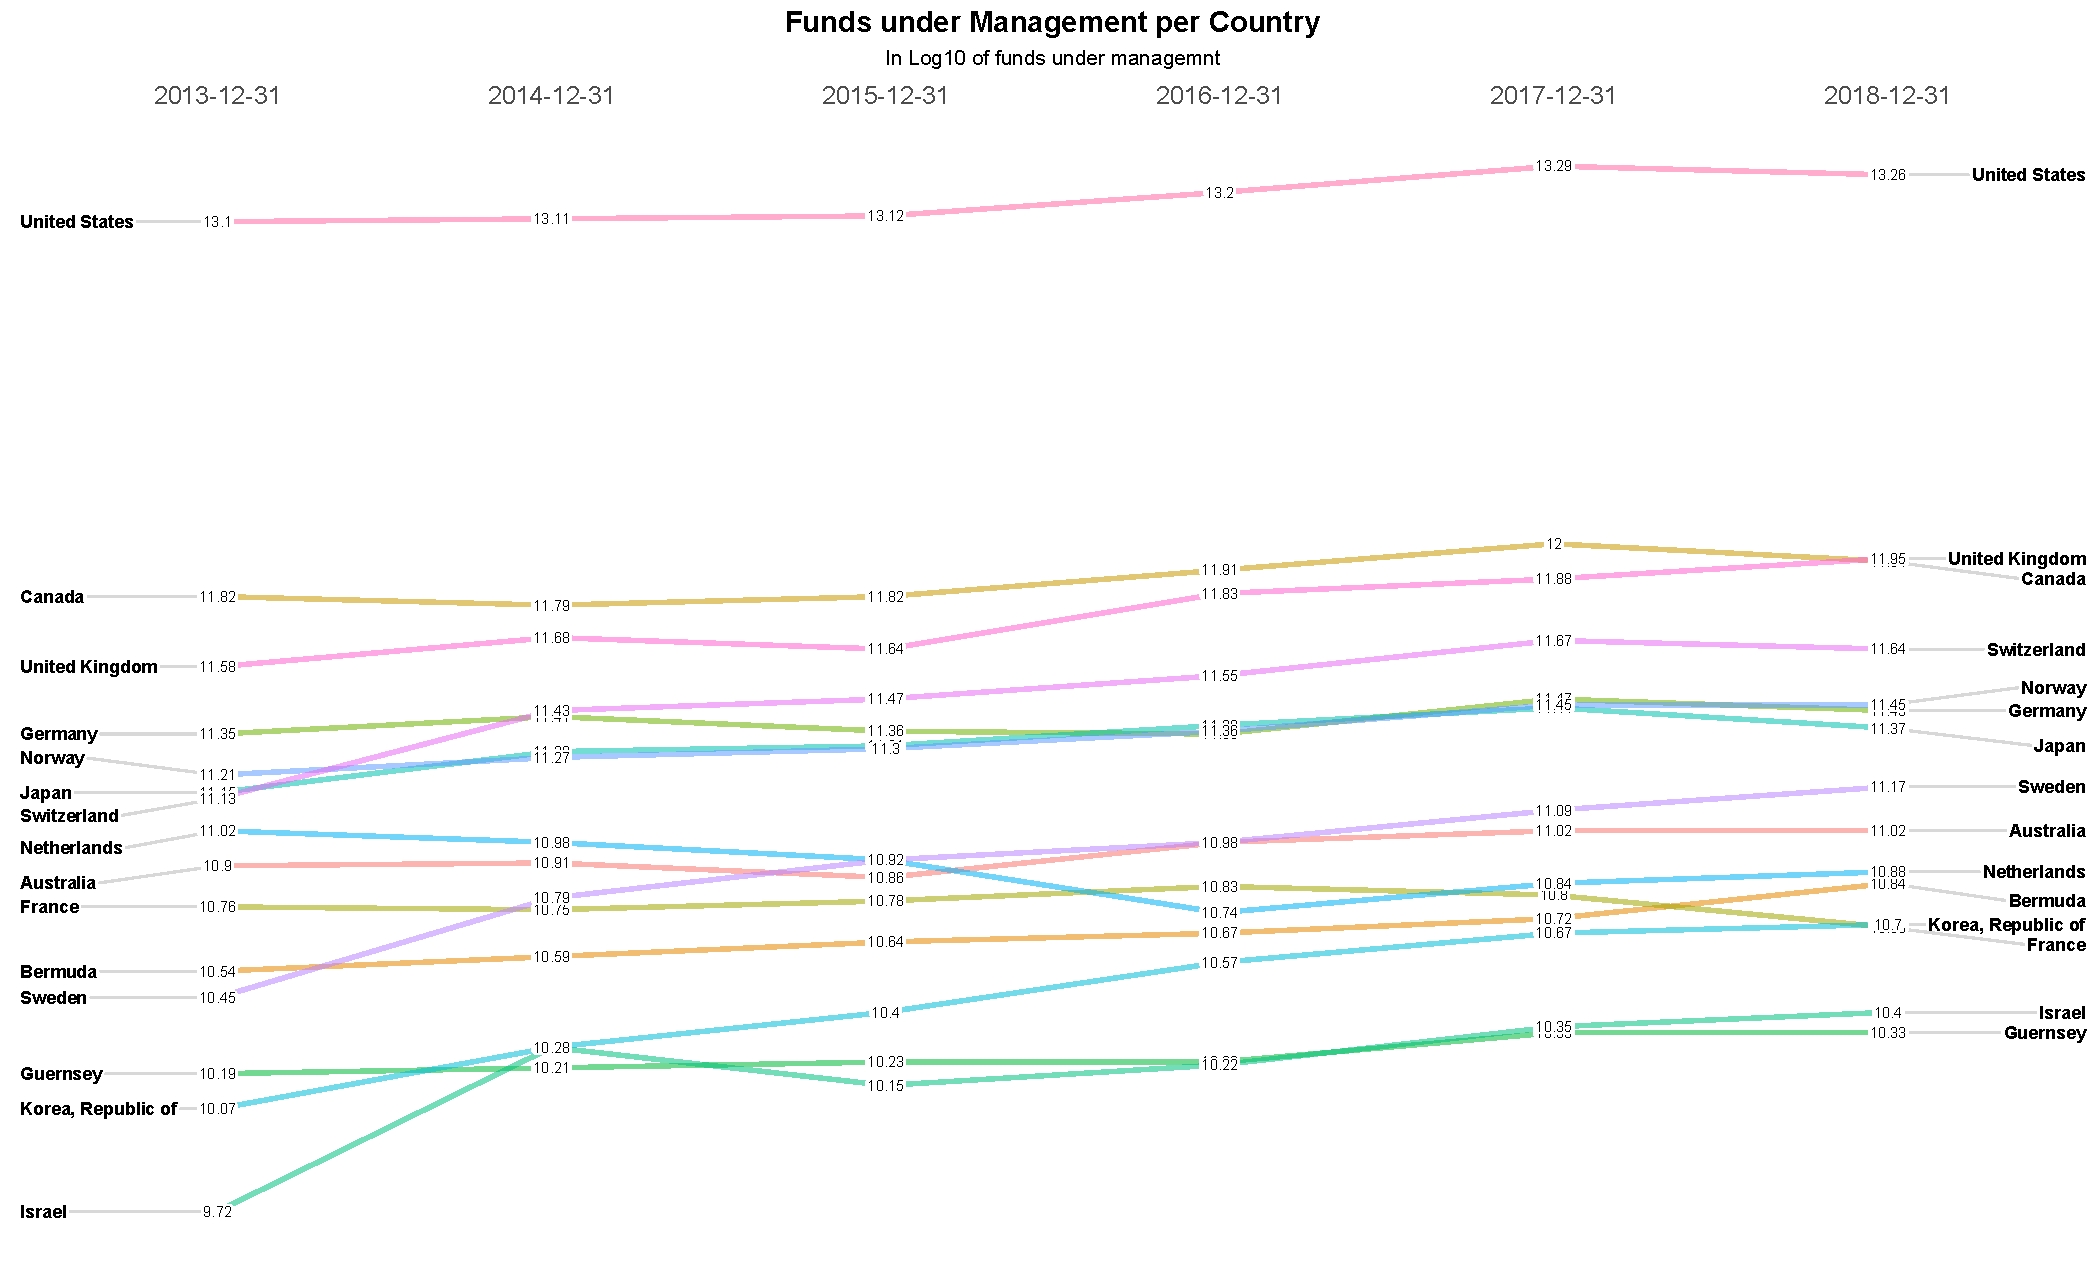
\includegraphics[width=1\linewidth]{Figures/ChapterIII/Funds_Per_Country_Slopegraph}
	\caption[Funds Under Management per Country in Log10]{Funds under management by country/political entity for top 15 countries in the world by funds under management.  Due to the very large gap between the USA and all other countries, the dollar value is represented in log10 form.}
	\label{fig:fundspercountryslopegraph}
\end{figure}


Figure \ref{fig:fundspercountryslopegraph} is a slope graph showing the sum of funds under management for all firms headquartered in each country.  As explored earlier, the 13F holdings report is a US legal instrument primarily interested in reporting the holdings of shares of US headquartered companies. It is no surprise that the United States of America is over-represented in this database.  Furthermore, since many of the other countries on this list have their own robust domestic stock markets, one should take caution before making direct comparison between the US-based investors and foreign investors.  Secondly, it is interesting to note that Canada, despite being a smaller economy than the United Kingdom, is home to more investors as measured by funds under management than UK based investors\footnote{This is strictly true provided that Crown Dependencies (Guernsey, Jersey, and the Isle of Mann) and British Overseas Territory (Gibraltar and Bermuda being the most prominent) are excluded from the UK's total.  With respect to the law, the Crown Dependencies are not part of the UK legislative and legal apparatus, and are autonomous with regard to their legal system, however the Crown is ultimately responsible for maintain good governance of these territories.  \citep{CrownDependencies}}. Finally, it is not surprising that the list of countries in Figure \ref{fig:fundspercountryslopegraph} are mostly populated by advanced economies and countries/political entities that specialise in financial services, such as Switzerland, Guernsey, and Bermuda.



\subsection{Investors By State}

While the 13F data has global reach with regards to foreign investors using US investment system, the use of domestic stock market is a significant confounding variable.  Therefore, for practical purposes, the focus of this research will be centred to a greater extent on the United States of America, its commonwealths and oversees territories.

\begin{figure}[h]
	\centering
	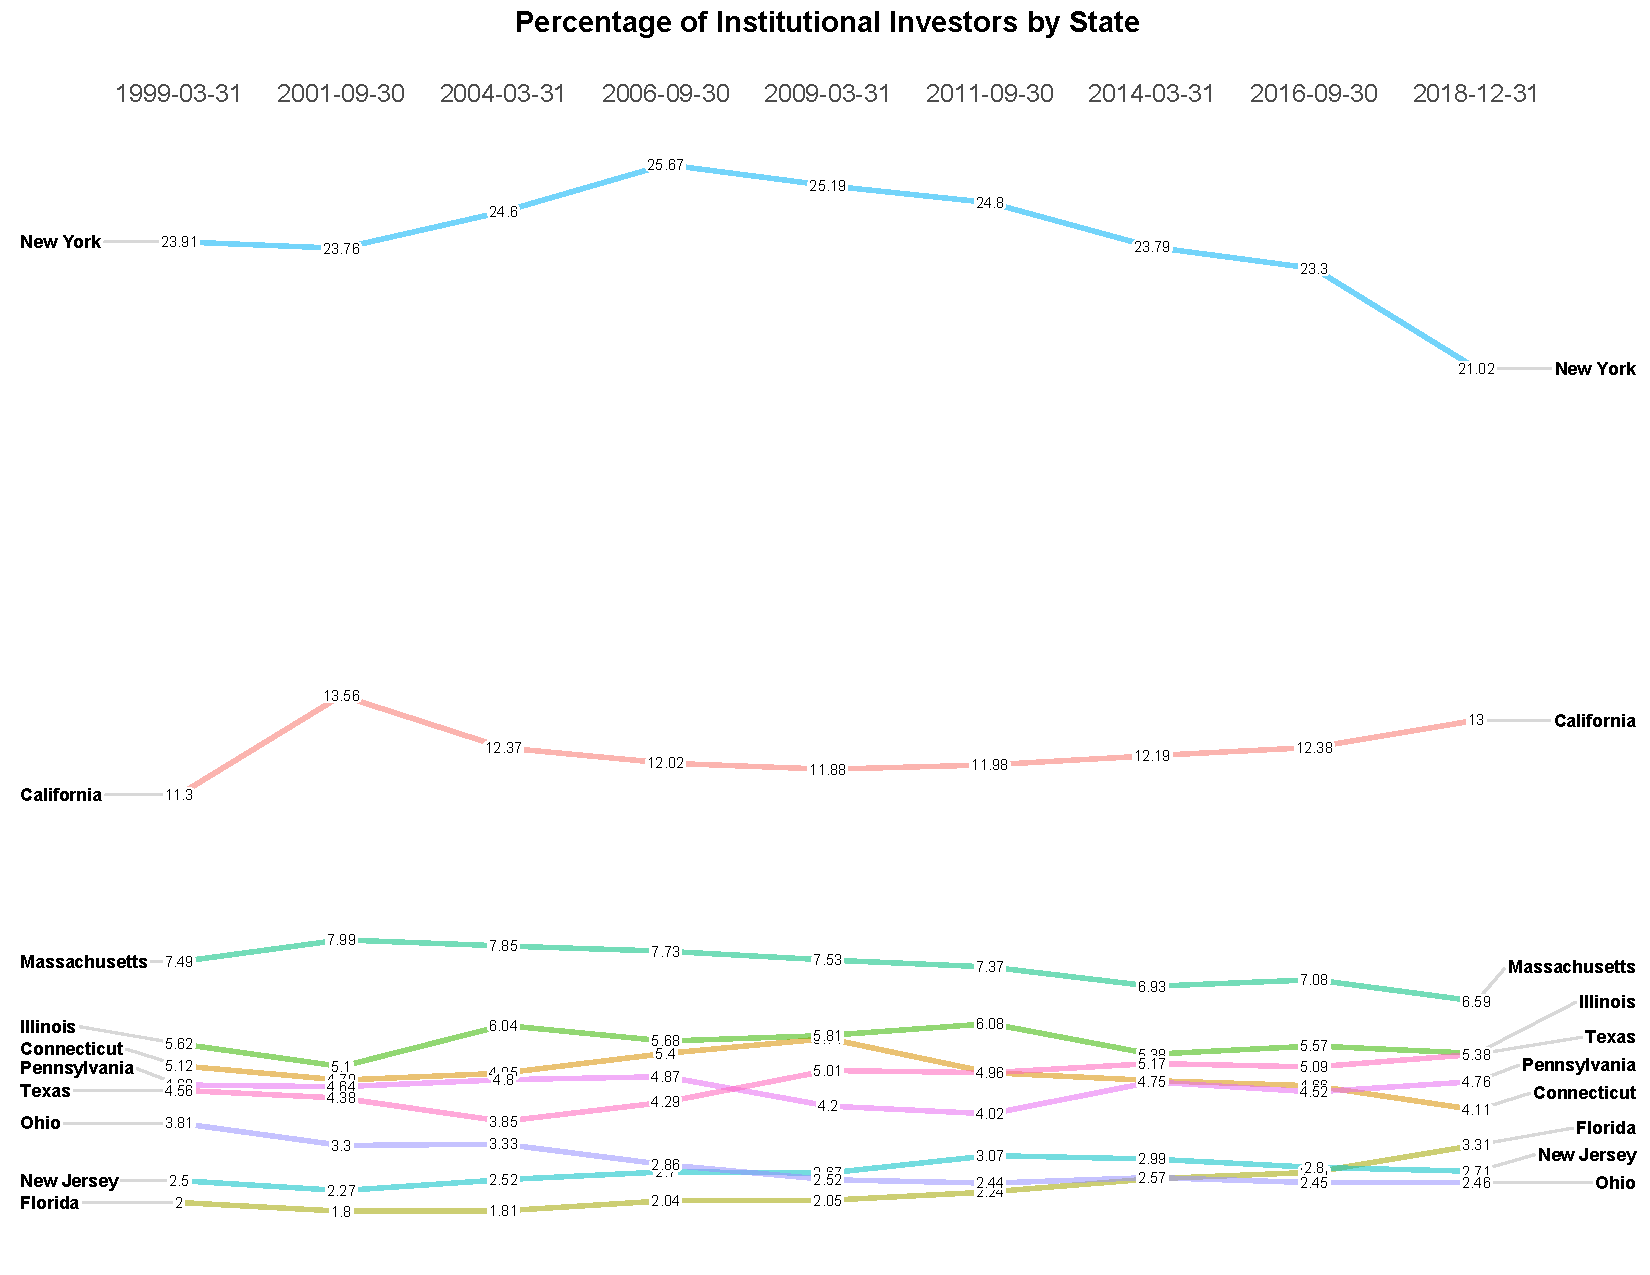
\includegraphics[width=\linewidth]{Figures/ChapterIII/Precentage_State}
	\caption[Percentage of Investor by State]{Percentage of institutional investors locational preference by share of investors by State.}
	\label{fig:precentagestate}
\end{figure}
There exists institutional investors in every US State, however there is a very unequal distribution when it comes to their location, by both number of investors and funds under management. \cite{WheelerMitchelson89,Green1995,bodenmanfirm2000, Graves2003} have seen and forecasted the continued relative decline of New York, and specifically it's namesake city.  And yet, despite the continual relative decline of New York State's position at the centre of the United States's financial system (Figure \ref{fig:precentagestate}), New York State is still home to the largest growth in institutional investors in absolute terms for this time period (Figure \ref{fig:countiibystate}). It should be noted that the renewal of New York's relative decline resumes on or around the first quarter of 2007.  This will be discussed in further detail at the county level (Section \ref{investorsbycounty}) and in point pattern analysis using Ripley's K (Section \ref{kfunction}).  	

\begin{figure}[h]
	\centering
	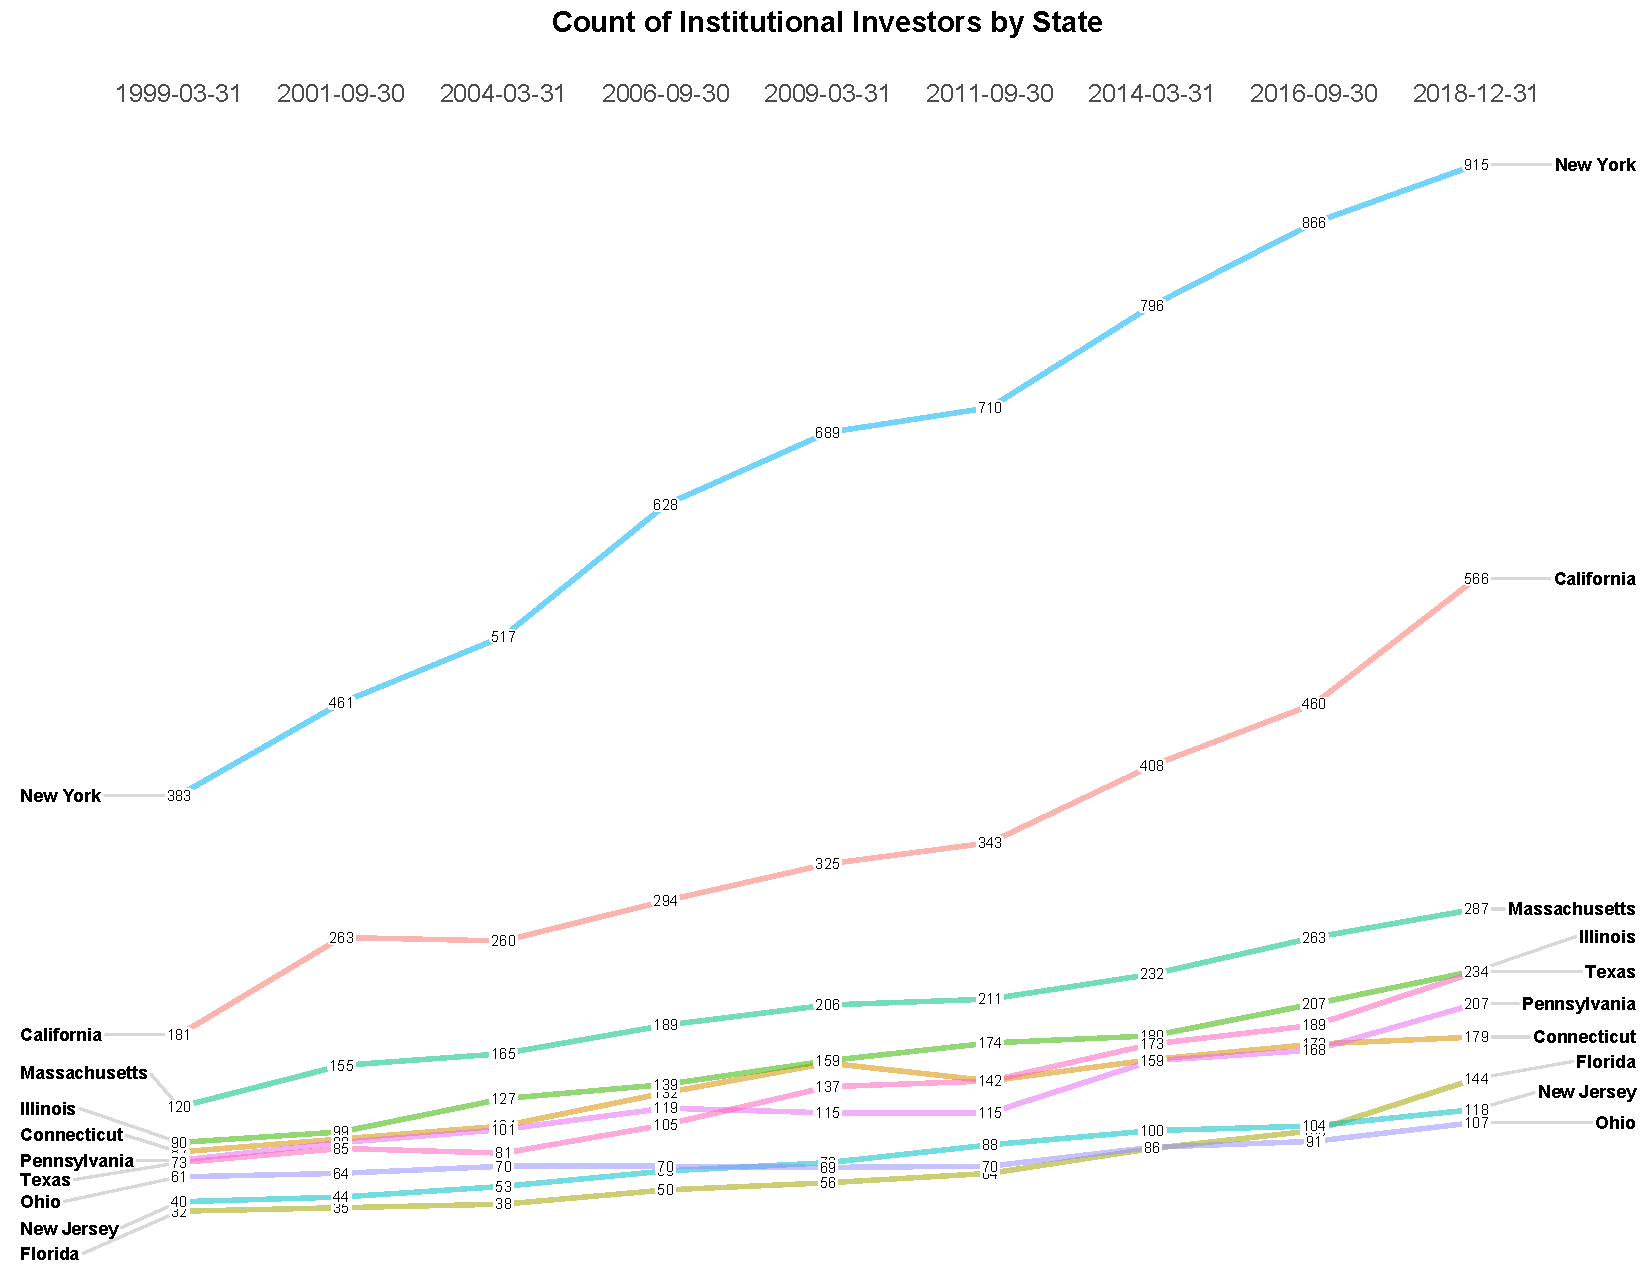
\includegraphics[width=1\linewidth]{Figures/ChapterIII/Count_II_BY_State}
	\caption[Count of Institutional Investors by State]{Count of institutional investors by State for the period 1999 to 2018.}
	\label{fig:countiibystate}
\end{figure}

While the region that contained the former industrial heart of the United States of America is experiencing a rather severe relative decline, these regions still manage to grow their number of firms in absolute terms.  This suggests that the cause of relative decline is a slower genesis of new firms rather than a migration of footloose firms.  This is consistent with the findings of \cite{gongthe2012}, which show that despite large shocks, a firm's geographical preferences are sticky.  

Further evidence for the point that firms are sticky can be found in figure \ref{fig:distancemovedhistogram}, where the great circle distance was measured between the locations of the first and second, second and third, third and fourth, ect... locations of firms in the ``phonebook'' database of 13F filers created by the author.  In the database there are 14 922 unique location and central index key (CIK)\footnote{Unique SEC identifier} combinations, of which 5 603 firms (CIK) stay in the same location for the duration.  For the remainder of 3 649 firms (CIKs), the database show them making 5 190 moves, for a total of 9 319 unique CIK/locations.  While this 9 319 unique locations may make the moves to appear very footloose, one must remember that a move implies two distinct locations.  In this database, the most footloose firm has a total of 7 moves, but this is the far end of the distribution as seen in Table \ref{tab:Numberofmoves}.  

% Table created by stargazer v.5.2.2 by Marek Hlavac, Harvard University. E-mail: hlavac at fas.harvard.edu
% Date and time: Thu, Feb 20, 2020 - 2:39:04 PM
\begin{table}[!htbp] \centering 
	\begin{tabular}{@{\extracolsep{5pt}} lccccccc} 
		\\[-1.8ex]\hline 
		\hline \\[-1.8ex] 
		Number of Moves & 1 & 2 & 3 & 4 & 5 & 6 & 7 \\ 
		\hline \\[-1.8ex] 
		Count & $2,477$ & $886$ & $221$ & $52$ & $9$ & $3$ & $1$ \\ 
		\hline \\[-1.8ex] 
	\end{tabular} 
	\caption[Number Moved by Firms]{Number of Moves by an institutional investor between the years 1999 and 2018}
	\label{tab:Numberofmoves}
\end{table} 

During this time period, 4 917 of 5 190 (94.7\%) of location changes have been what can be considered intra-city/intra-metro area (less than 150 km) rather than 
47 inter-city.  This lack of long-distance movement makes attracting firms to a new locale a near-non factor in location changes over time, suggesting some costs in movement, or that rent isn't a top-line deciding factor in location.  Even more important for how sticky firms are in their locational preference are that 2 903 of 5 190 (55.9\% ) of firm locational changes are of less than 1 km in distance.

One would be remiss to not point out that movement can evade capture in this data set by closing down firm A in location Alpha and creating firm B in location Beta.  However, since this would necessitate a non-negligible amount of paperwork, it is doubtful that this would occur only for the purpose of concealing changes in location.   

\nomenclature{CIK}{Central Index Key}

\begin{figure}
	\centering
	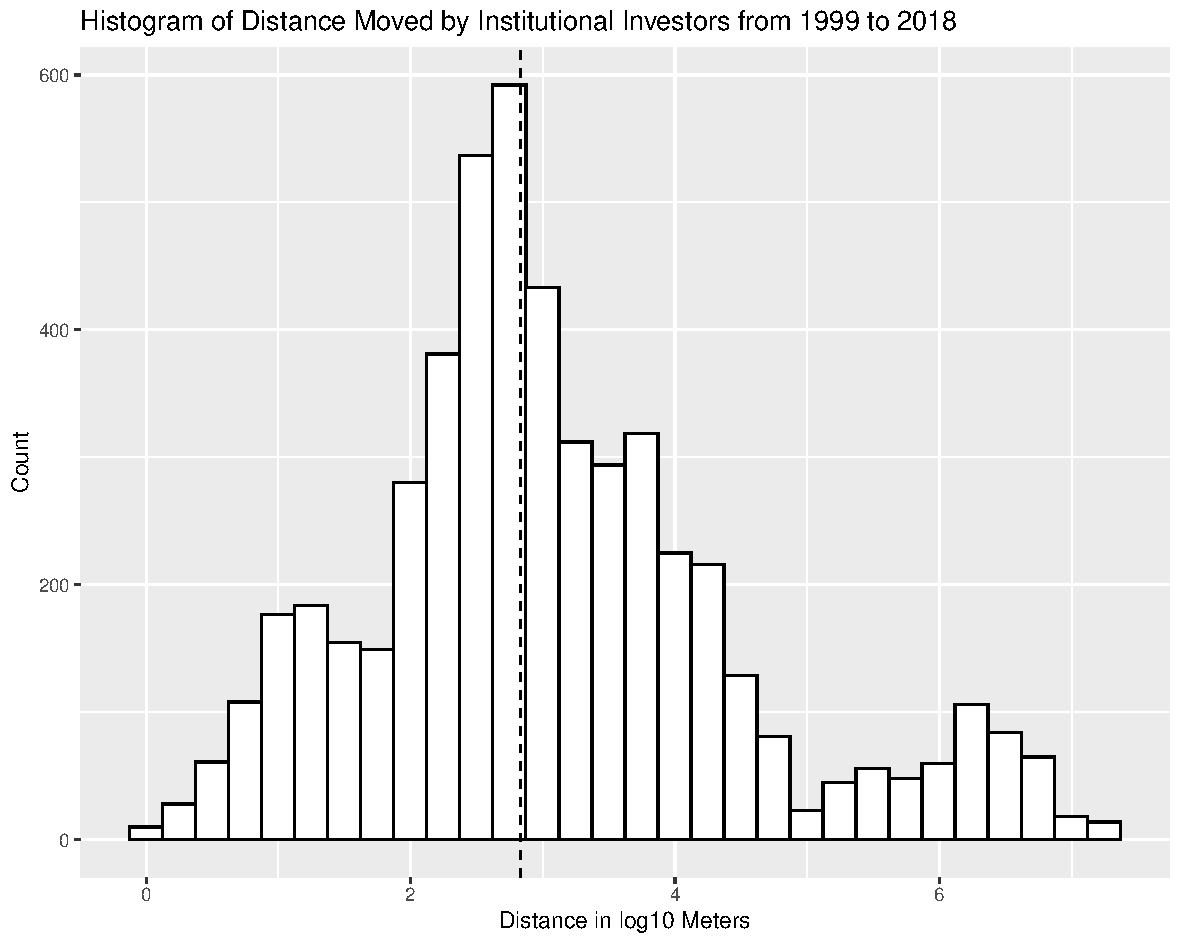
\includegraphics[width=0.7\linewidth]{Figures/ChapterIII/Distance_Moved_Histogram}
	\caption[Distance Moved by Firms]{Distance Moved by firms during the time period of 1999 to 2018 in Log10 meters.  The dashed vertical bar represents the median distance traveled of 680 meters.  The mean distance was 269 040 meters.  (All distances rounded to the nearest 10m).}
	\label{fig:distancemovedhistogram}
\end{figure}

A further cause for the widespread distribution of institutional investors in the United States is the historical legacy of US banking regulations.  The 10th Amendment of the US Constitution reserved banking regulations to the States, whereas the commerce clause gave the Federal government jurisdiction over interstate commerce.  This division in jurisdiction led to the creation of a regime of regional banks rather than a small clique of national banks \citep{Calomiris2000}. Furthermore, the proliferation of State-managed employee pension funds ensures the existence of institutional investors outside of financially centred metropolitan areas such as New York, Boston, Chicago or San Francisco.  This remains the case despite the recent trend of outsourcing a sizable portions of pension funds into more opaque (and thus outside of the purview of 13F disclosure) and hopefully high yielding private placement deals \cite{lerner2019investing}. 




\subsection{Investors by Core-Based Statistical Area}


\nomenclature{CBSA}{Core-Based Statistical Area}
Core-Based Statistical Areas (CBSA) are a relatively recent geographical construct by the U.S. Office of Management and Budget with the goal of creating a set of nationally consistent geographies that are useful for tabulating and comparing statistics.  These areas consist of at least one core county with a population greater than 10 000 inhabitants, as well as all adjacent counties with substantial economic and social integration \citep{USCensusCBSAdef}.  The CBSA is a useful construct for comparing urban areas since it creates a more homogeneous unit of comparison between different urban areas in the United States, particularly since the USA has a disparate mix of regional sub-units such as New England townships and Louisiana parishes.  Furthermore, the CBSA is subdivided into either a Metropolitan Statistical Area (population greater than 50 000) or a Micropolitan Statistical Area (population less than 50 000).  

Figure \ref{fig:countbycbsalegal} illustrates the absolute count of institutional investors by CBSA.  As previously mentioned in the State breakdown of institutional investors, the New York - Newark - Jersey City CBSA gains the largest absolute amount of new institutional investors by a considerable margin, and Figure \ref{fig:percentageofinvestmentfirmsbycbsa} shows a similar picture to Figure \ref{fig:precentagestate} in which New York sees a relative decline.  Due to the presence of a few investors in non-CBSA counties, the investors located outside of CBSA were added to figures \ref{fig:countbycbsalegal} and \ref{fig:percentageofinvestmentfirmsbycbsa}.  Of particular note is the rapid rise of investment firms outside of the USA during this time period.  Figure \ref{fig:percentageoffirmsbycbsa} is similar to Figure \ref{fig:percentageofinvestmentfirmsbycbsa}, but with the absence of foreign investment firms. When comparing these graphs, the difference in slope trajectory when the number of foreign firms is removed from the baseline is remarkable.   At this scale, the relative density of investment firms still follows the same inverted U shape, with a peak on or about the first quarter of 2007.  

\begin{figure}[h]
	\centering
	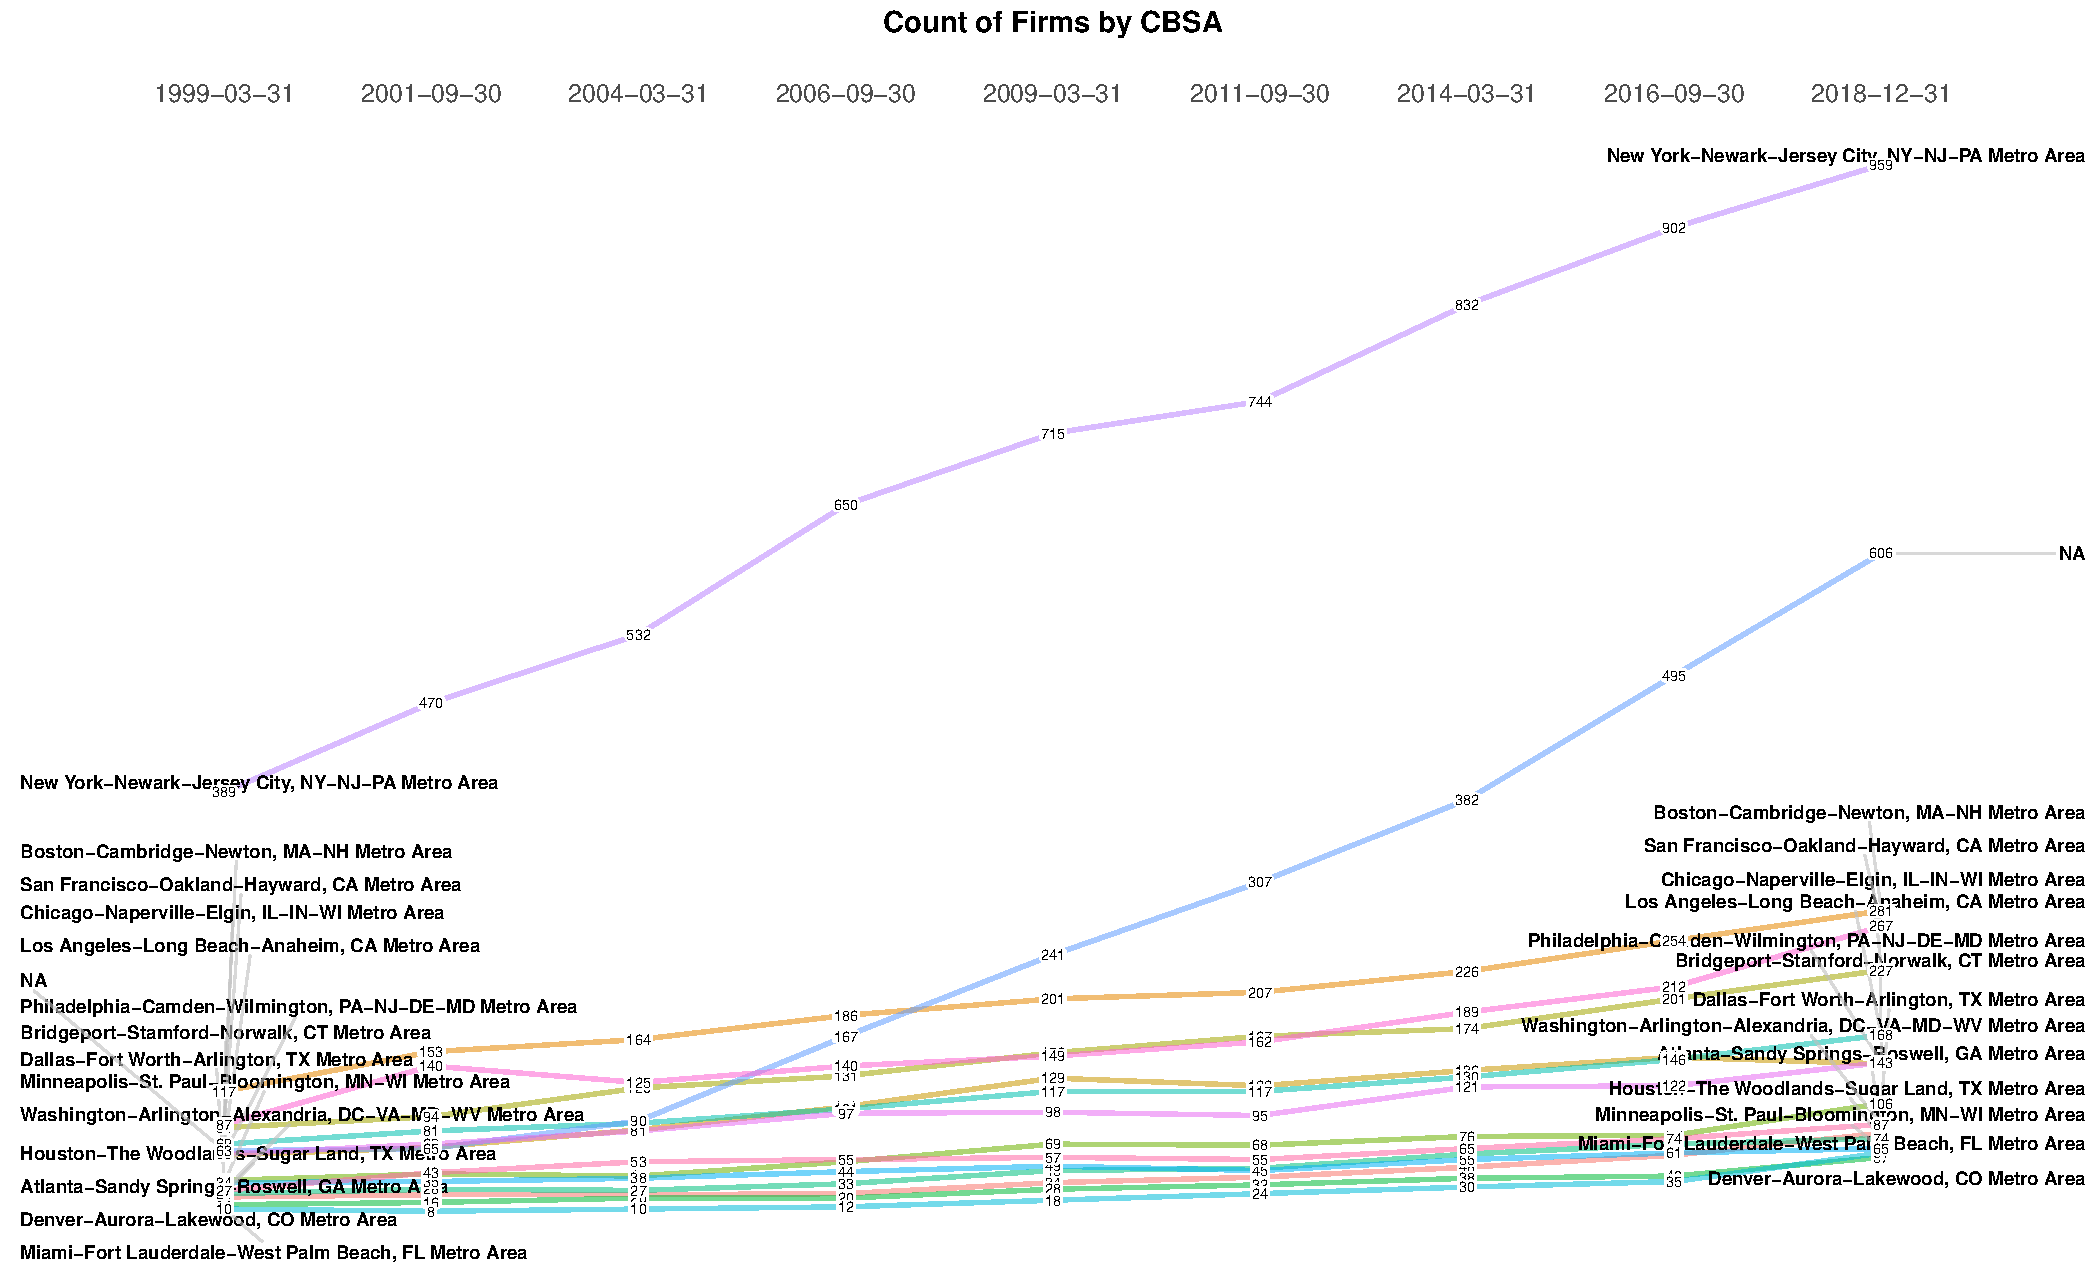
\includegraphics[width=1\linewidth]{Figures/ChapterIII/Count_by_CBSA_Legal}
	\caption[Count of Institutional Investors by CBSA]{Count of institutional investors by Core-Based Statistical Areas for the period 1999 to 2018}
	\label{fig:countbycbsalegal}
\end{figure}


\begin{figure}[h]
	\centering
	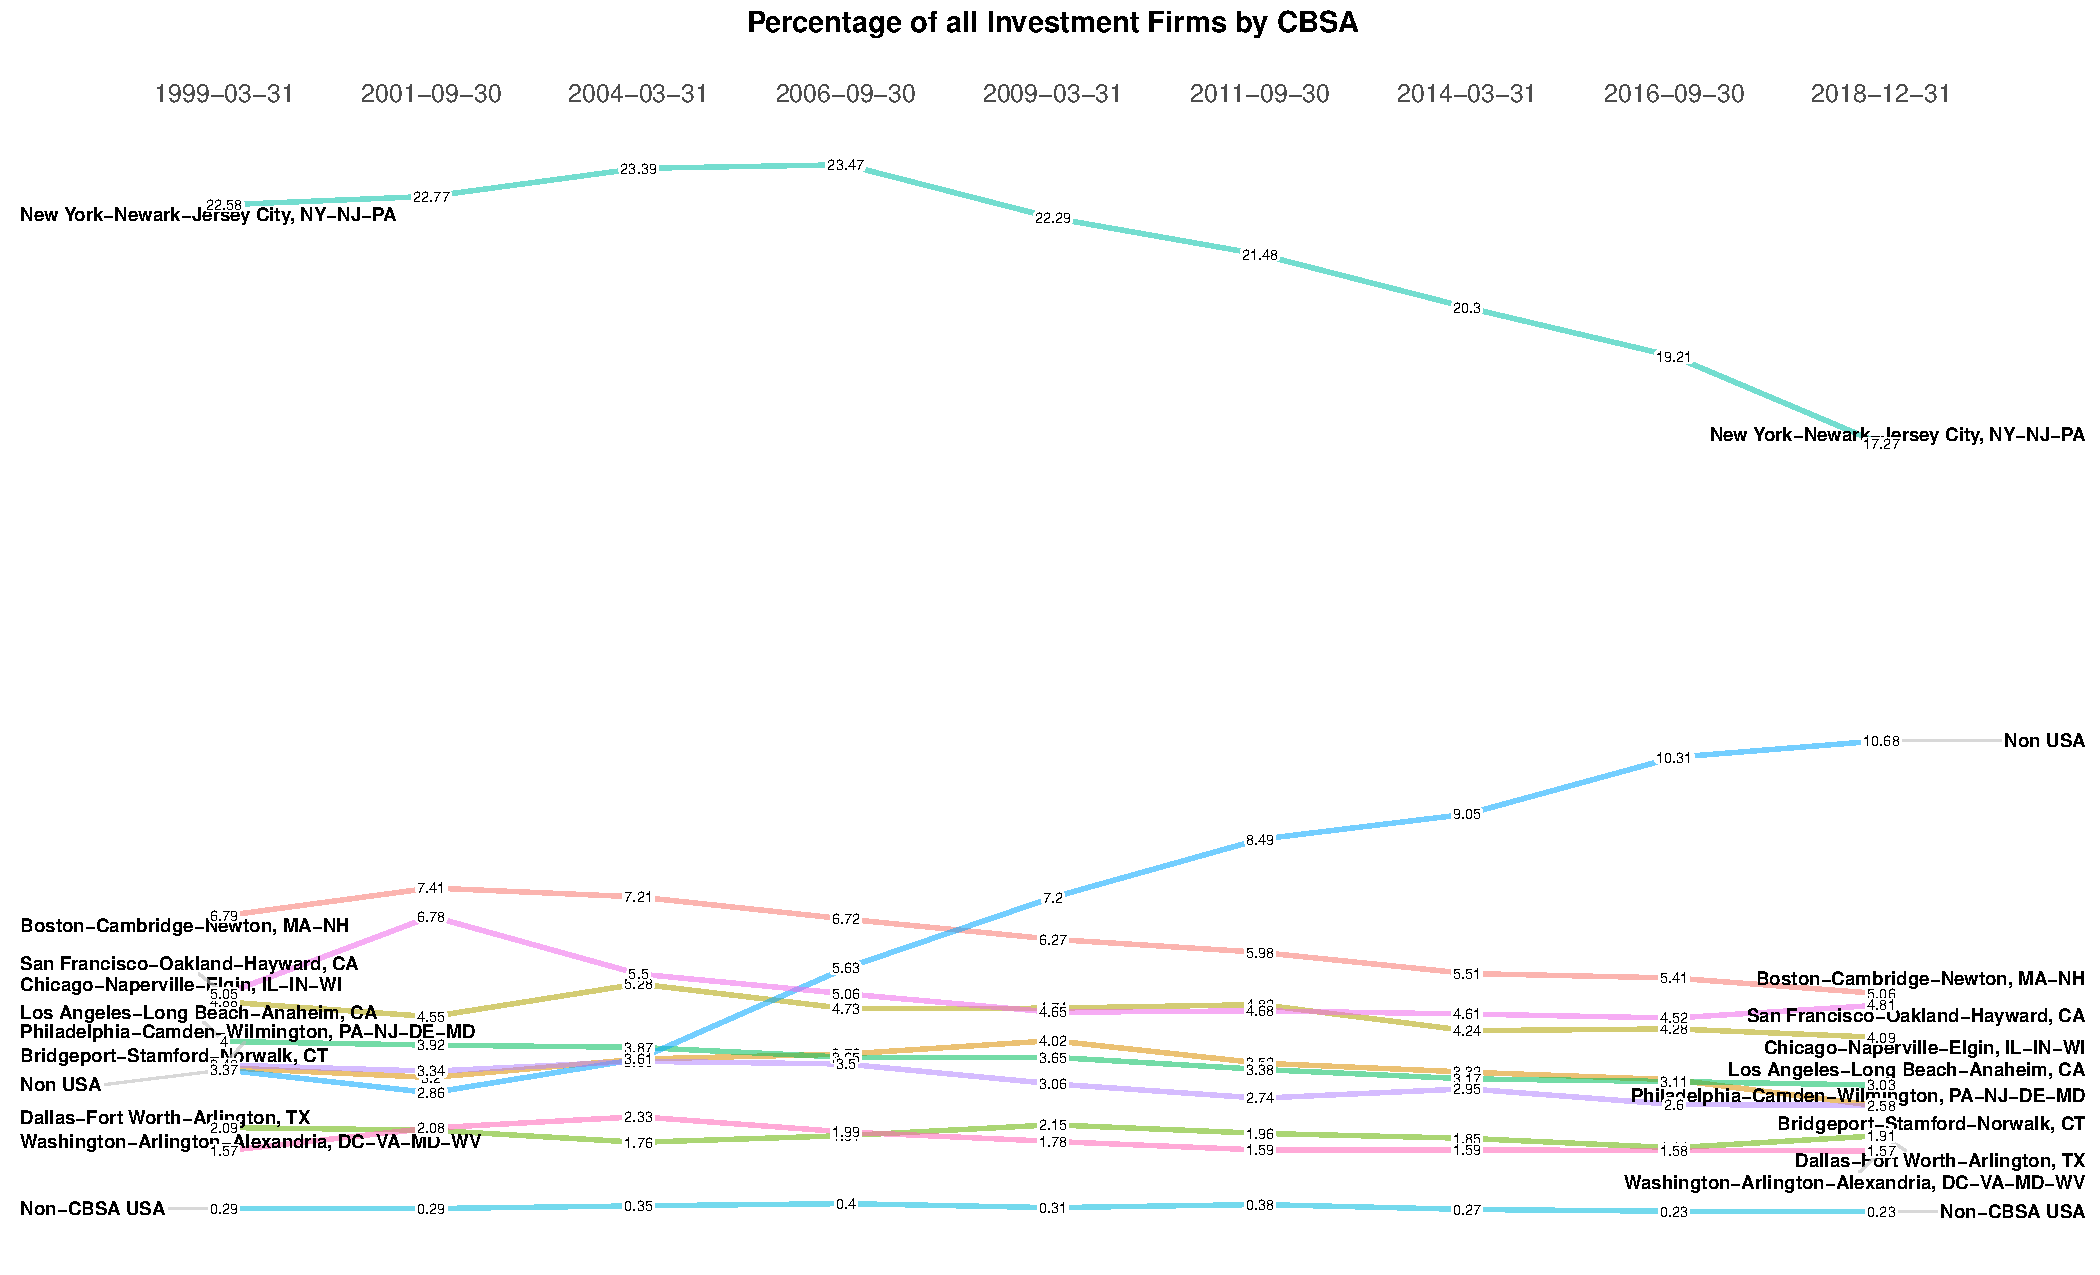
\includegraphics[width=1\linewidth]{Figures/ChapterIII/Percentage_of_Investment_Firms_by_CBSA}
	\caption[Share of Institutional Investors by CBSA]{Share of institutional investors by Core-Based Statistical Areas for the period 1999 to 2018}
	\label{fig:percentageofinvestmentfirmsbycbsa}
\end{figure}



\begin{figure}
	\centering
	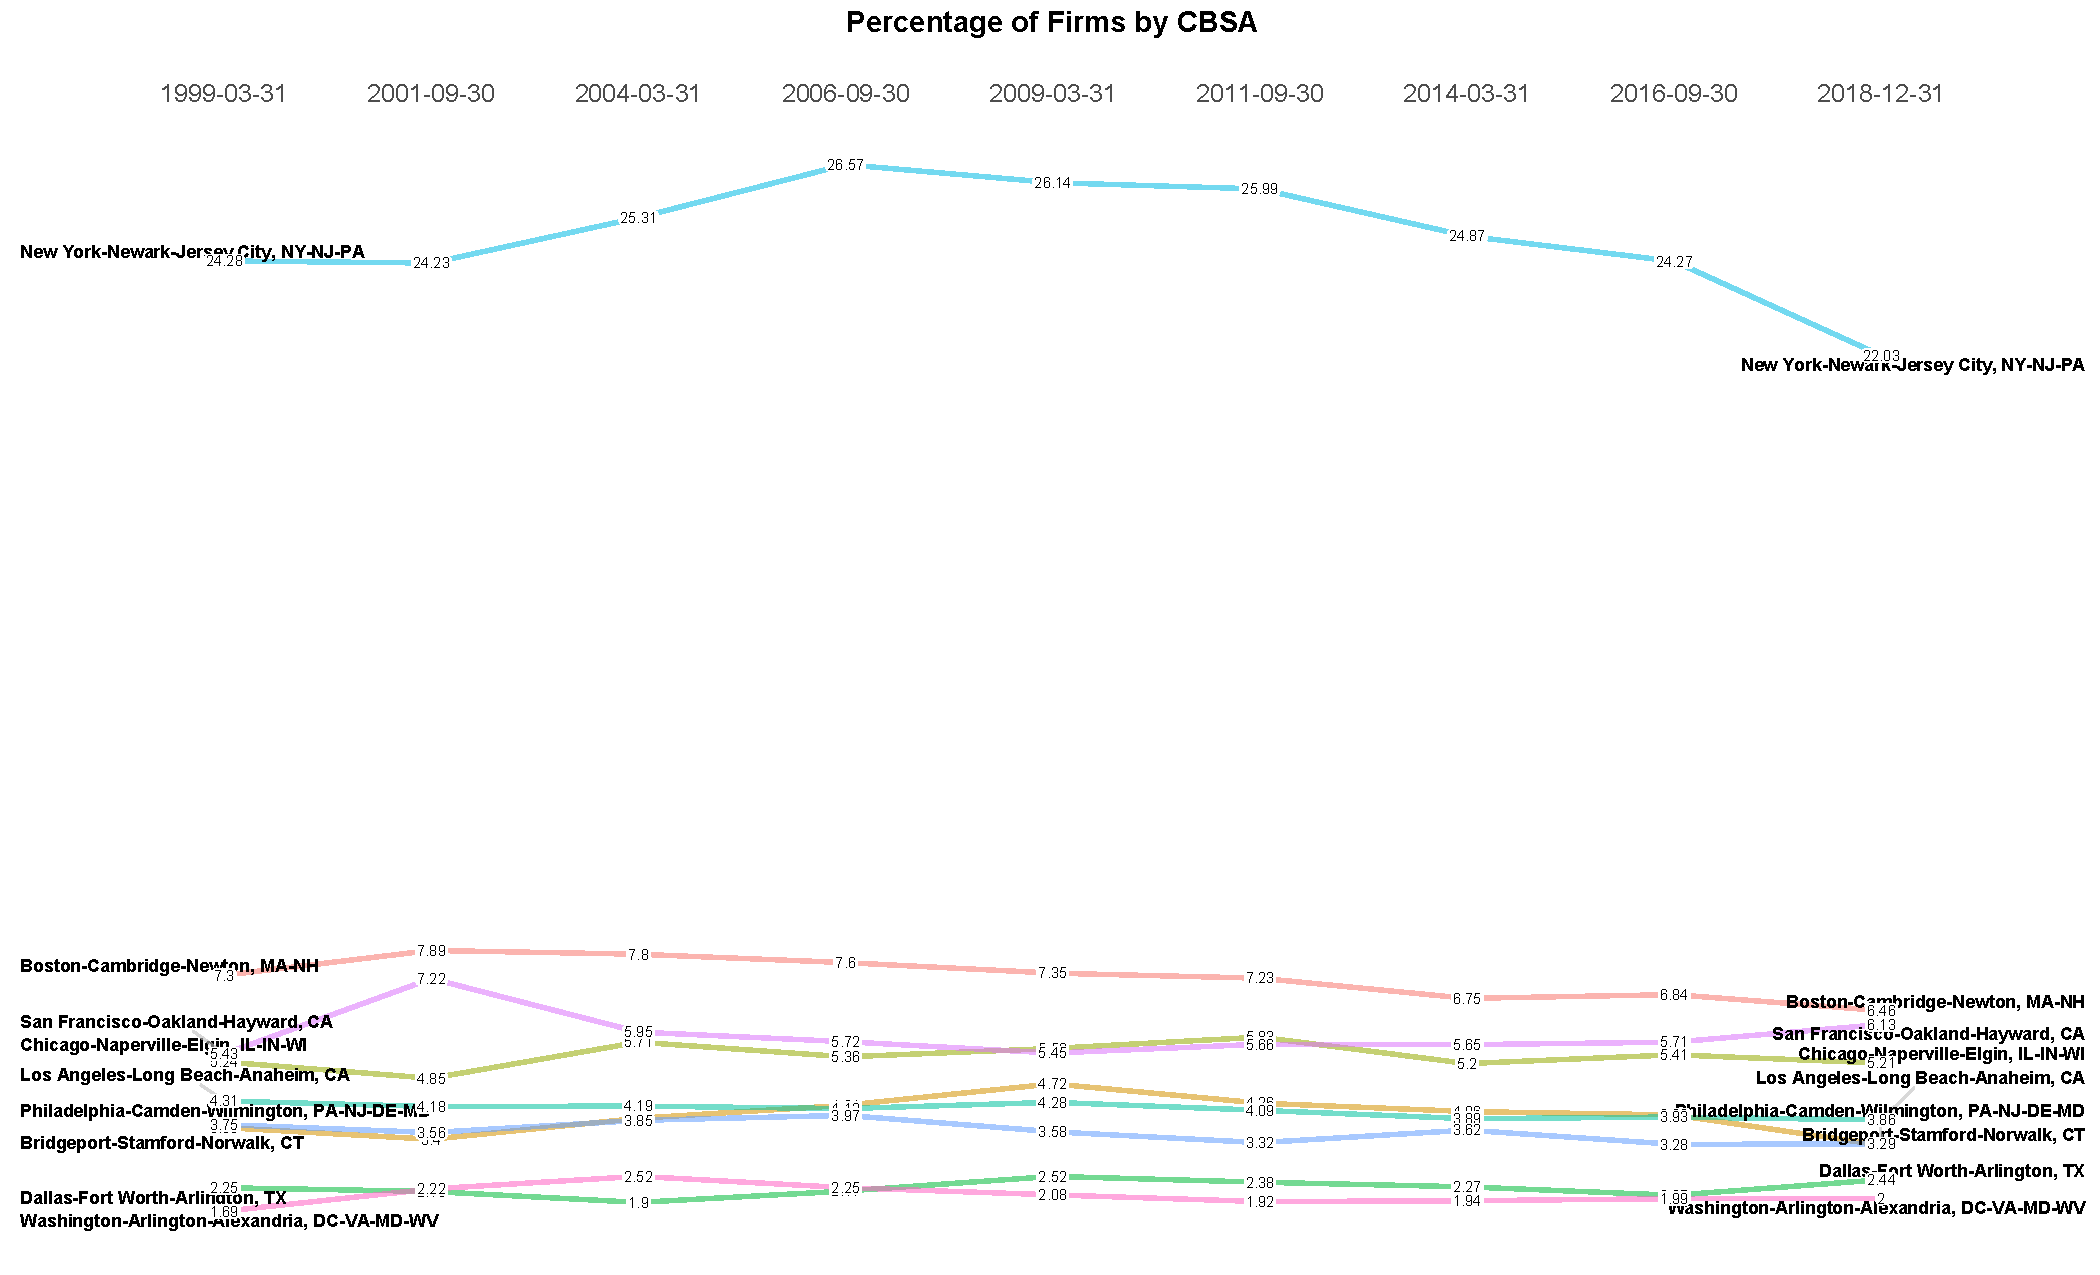
\includegraphics[width=1\linewidth]{Figures/ChapterIII/Percentage_of_Firms_by_CBSA}
	\caption[Percent by Share of Institutional Investors CBSA]{Percent by Share of institutional investors by Core-Based Statistical Areas for the period 1999 to 2018. Percentages are re-calibrated by removing investors located outside of CBSAs}
	\label{fig:percentageoffirmsbycbsa}
\end{figure}



\subsection{Investors by County}
\label{investorsbycounty}
Diving further down the building blocks of US territorial systems, the next level down is that of the county. There are 3 242 counties and county equivalents in the USA, and its territories,  of which 2 707 do not have institutional investors during the entire period. In March of 1999, 2 972 counties do not host an institutional investor, however by December 2018 the number of counties devoid of institutional investors falls to 2 786.  Considering that the USA added over 2 500 institutional investors during this period, this suggests that new institutional investors are attracted to counties with a pre-existing institutional investor population rather than filling-out empty counties.  



\begin{figure}
	\centering
	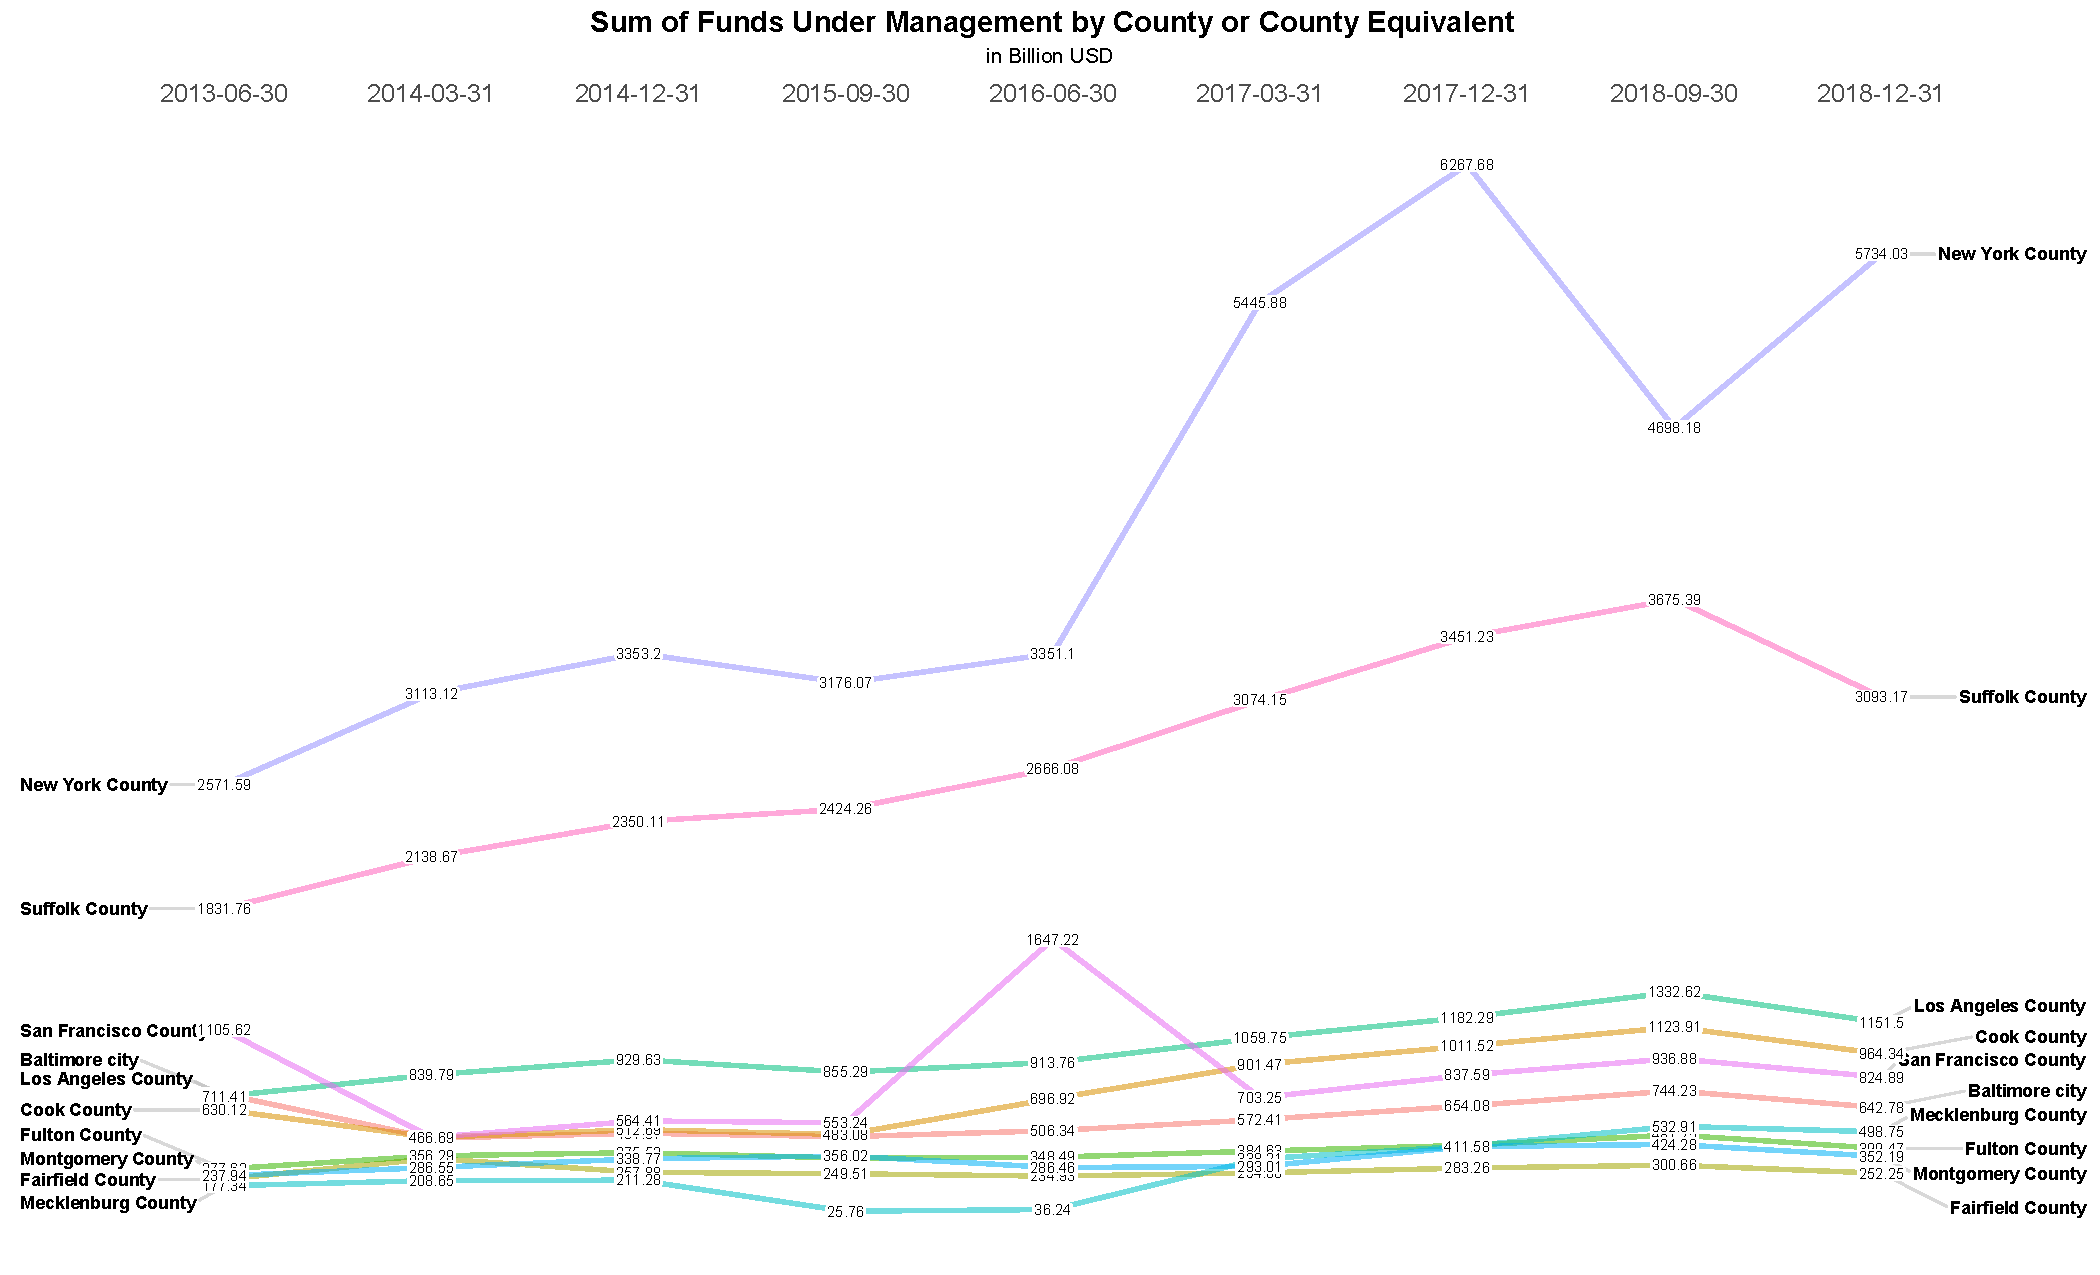
\includegraphics[width=1\linewidth]{Figures/ChapterIII/Sum_by_County}
	\caption[Sum of Institutional Investors by County]{Sum of institutional investors by county for the period 1999 to 2018}
	\label{fig:sumbycounty}
\end{figure}


\begin{figure}
	\centering
	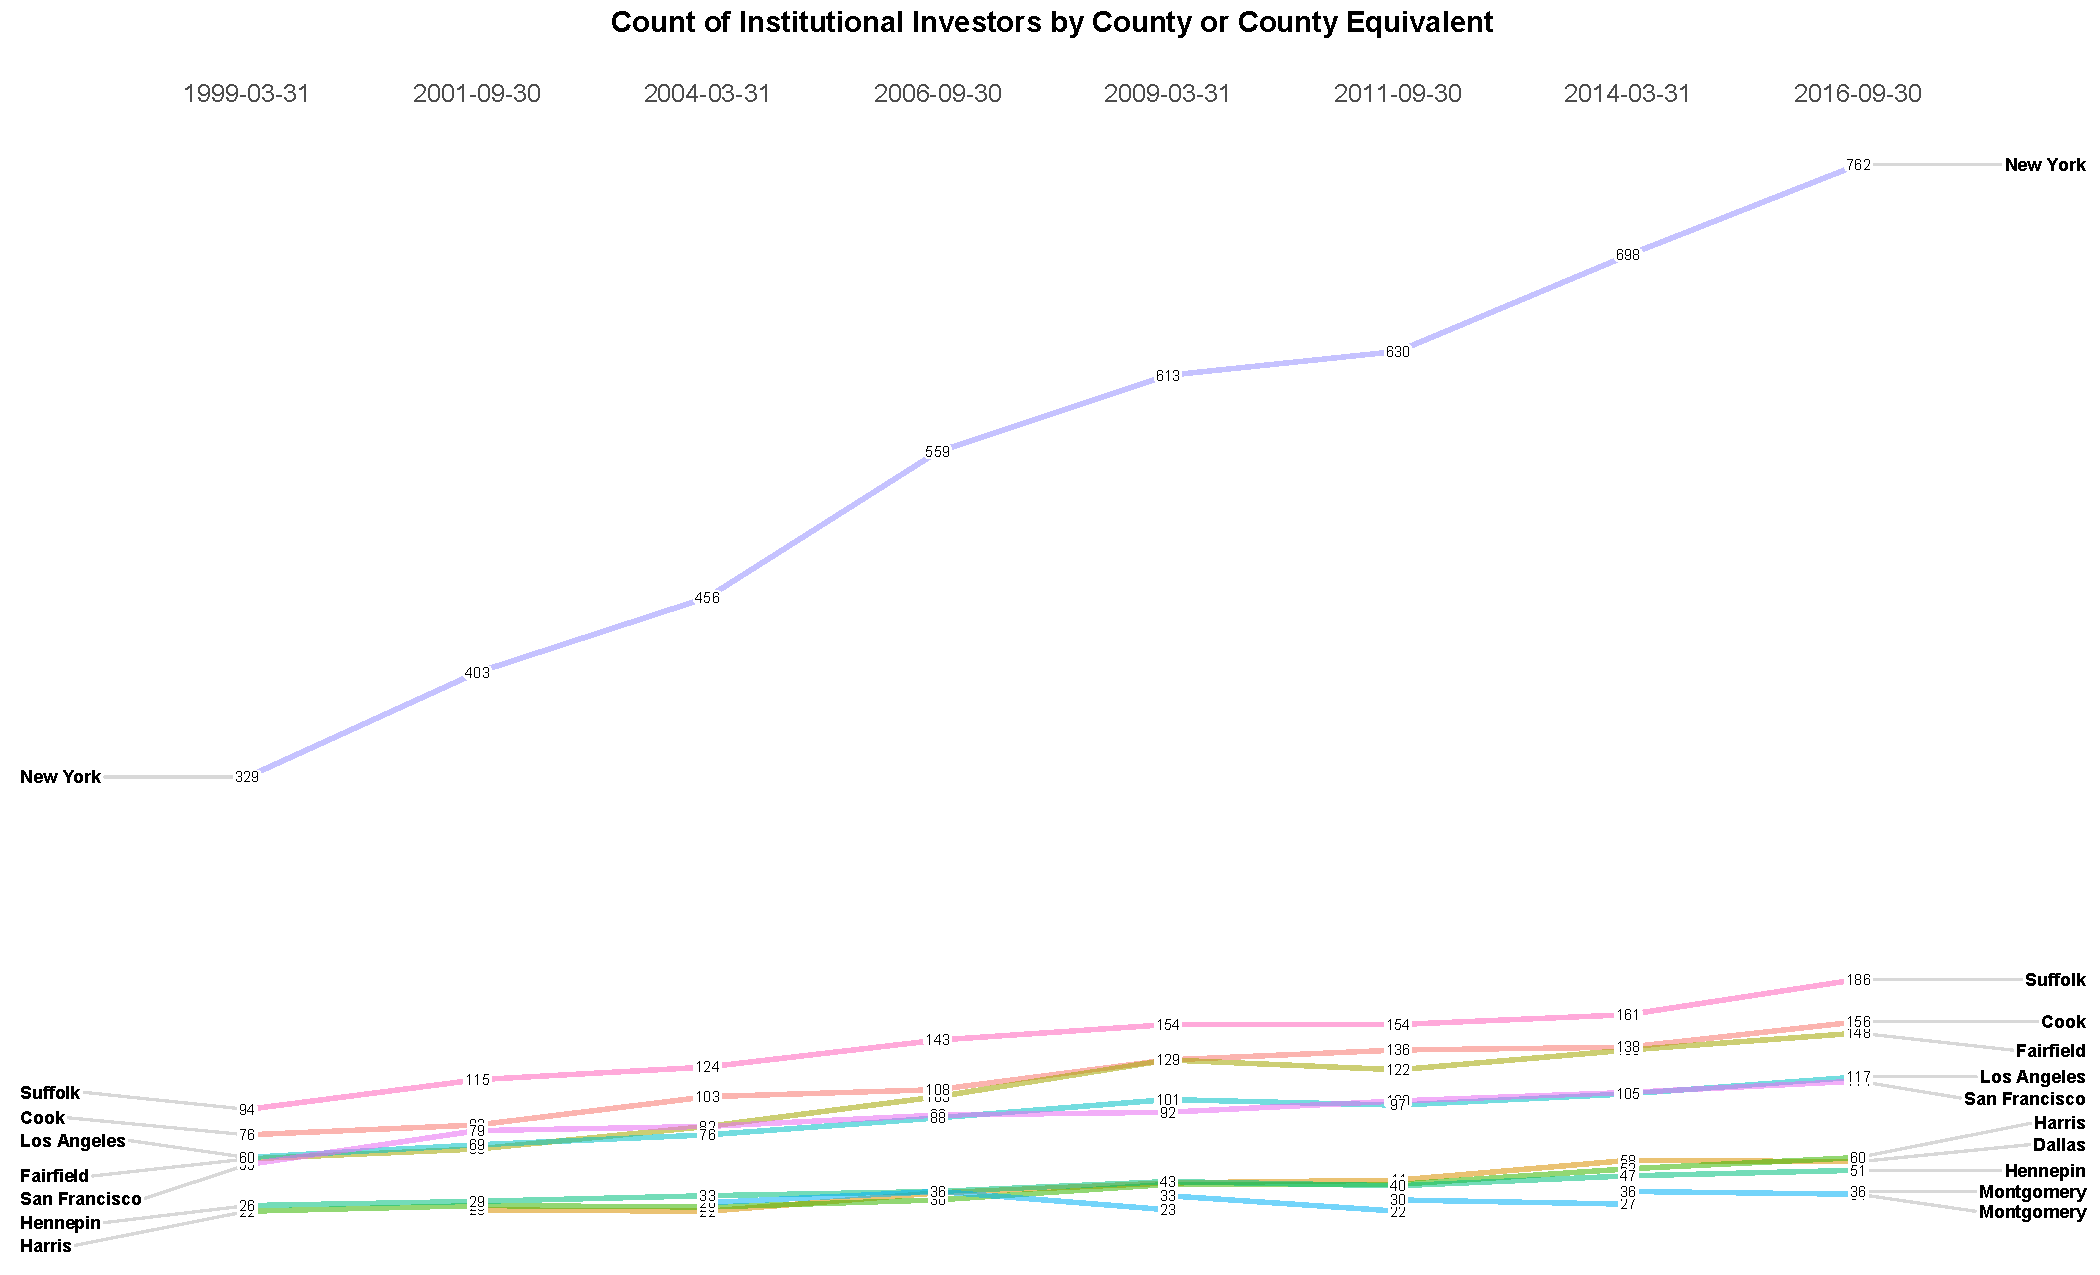
\includegraphics[width=1\linewidth]{Figures/ChapterIII/Count_by_County}
	\caption[Count  of Institutional Investors by County]{Count institutional investors by county for the period 1999 to 2018}
	\label{fig:countbycounty}
\end{figure}

This larger number of counties permits a different sort of analysis to be used: that of comparing Gini coefficients over time.  The Gini coefficient is a common descriptive statistic of inequality, with a value of 1 describing perfect inequality (one case having all of the measured variable) and 0 describing perfect equality (all cases having equal amounts of the variable). 

The Chow test is a statistical test developed by econometrician Gregory Chow for determining if two regression lines are equal.  Within the field of time series analysis, this is useful for determining if there is the presence of a structural break in the data.  	A look at figure \ref{fig:ginicounty} shows an increase in spatial dispersion over time.  Using a Chow test  (Figure \ref{fig:Chow Test}) to find the change in linear trend of the Gini coefficient indicates that there is a breakpoint in trend on June 30th, 2011  \citep{Chow1960}.  This is much later than the breakpoints mentioned earlier when looking at the concentration of firms in States and CBSAs. 	This can be somewhat explained by the Gini coefficient being more sensitive to areas going from 0 to 1 than say 15 to 16.  




\begin{figure}[h]
	\centering
	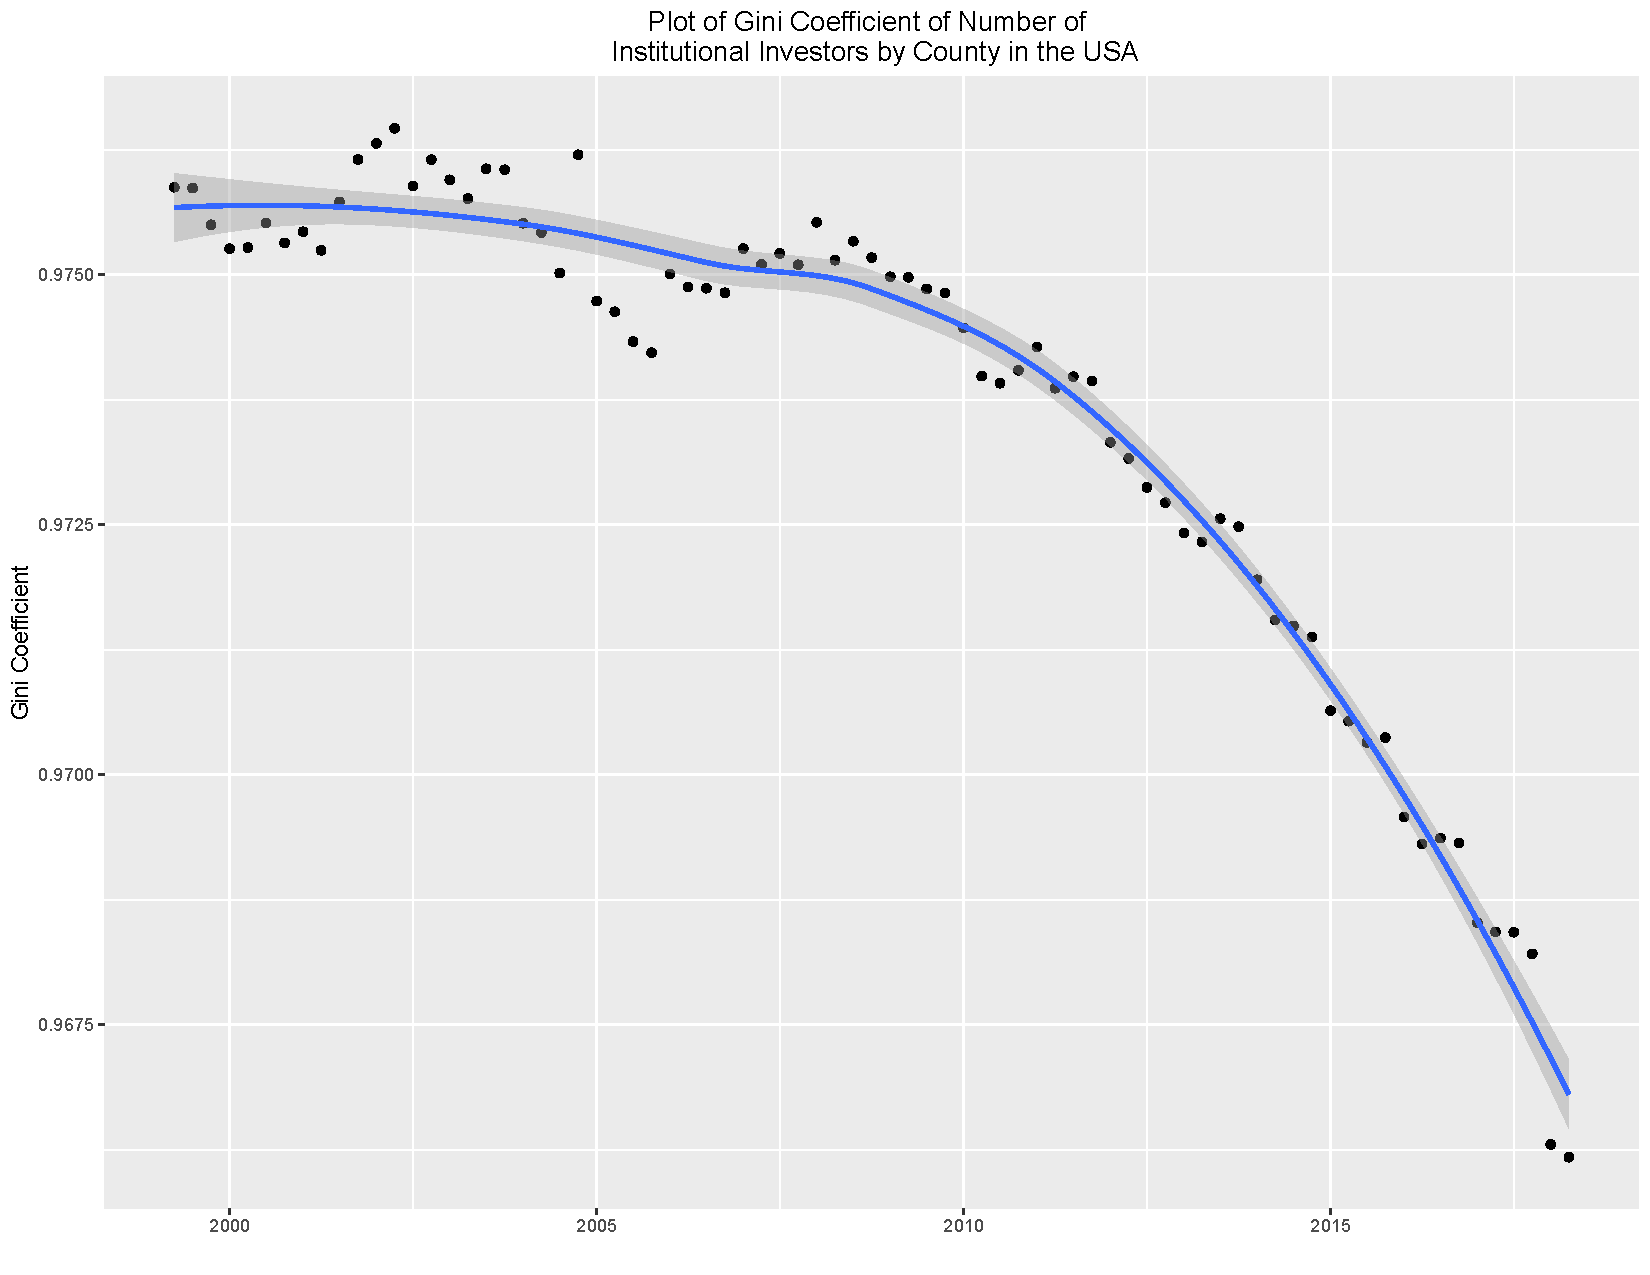
\includegraphics[width=1\textwidth]{Figures/ChapterIII/GINI_County}
	\caption[Gini Coefficient of US County Count]{Gini coefficient of US county count}
	\label{fig:ginicounty}
\end{figure}


\begin{figure}[h]
	\centering
	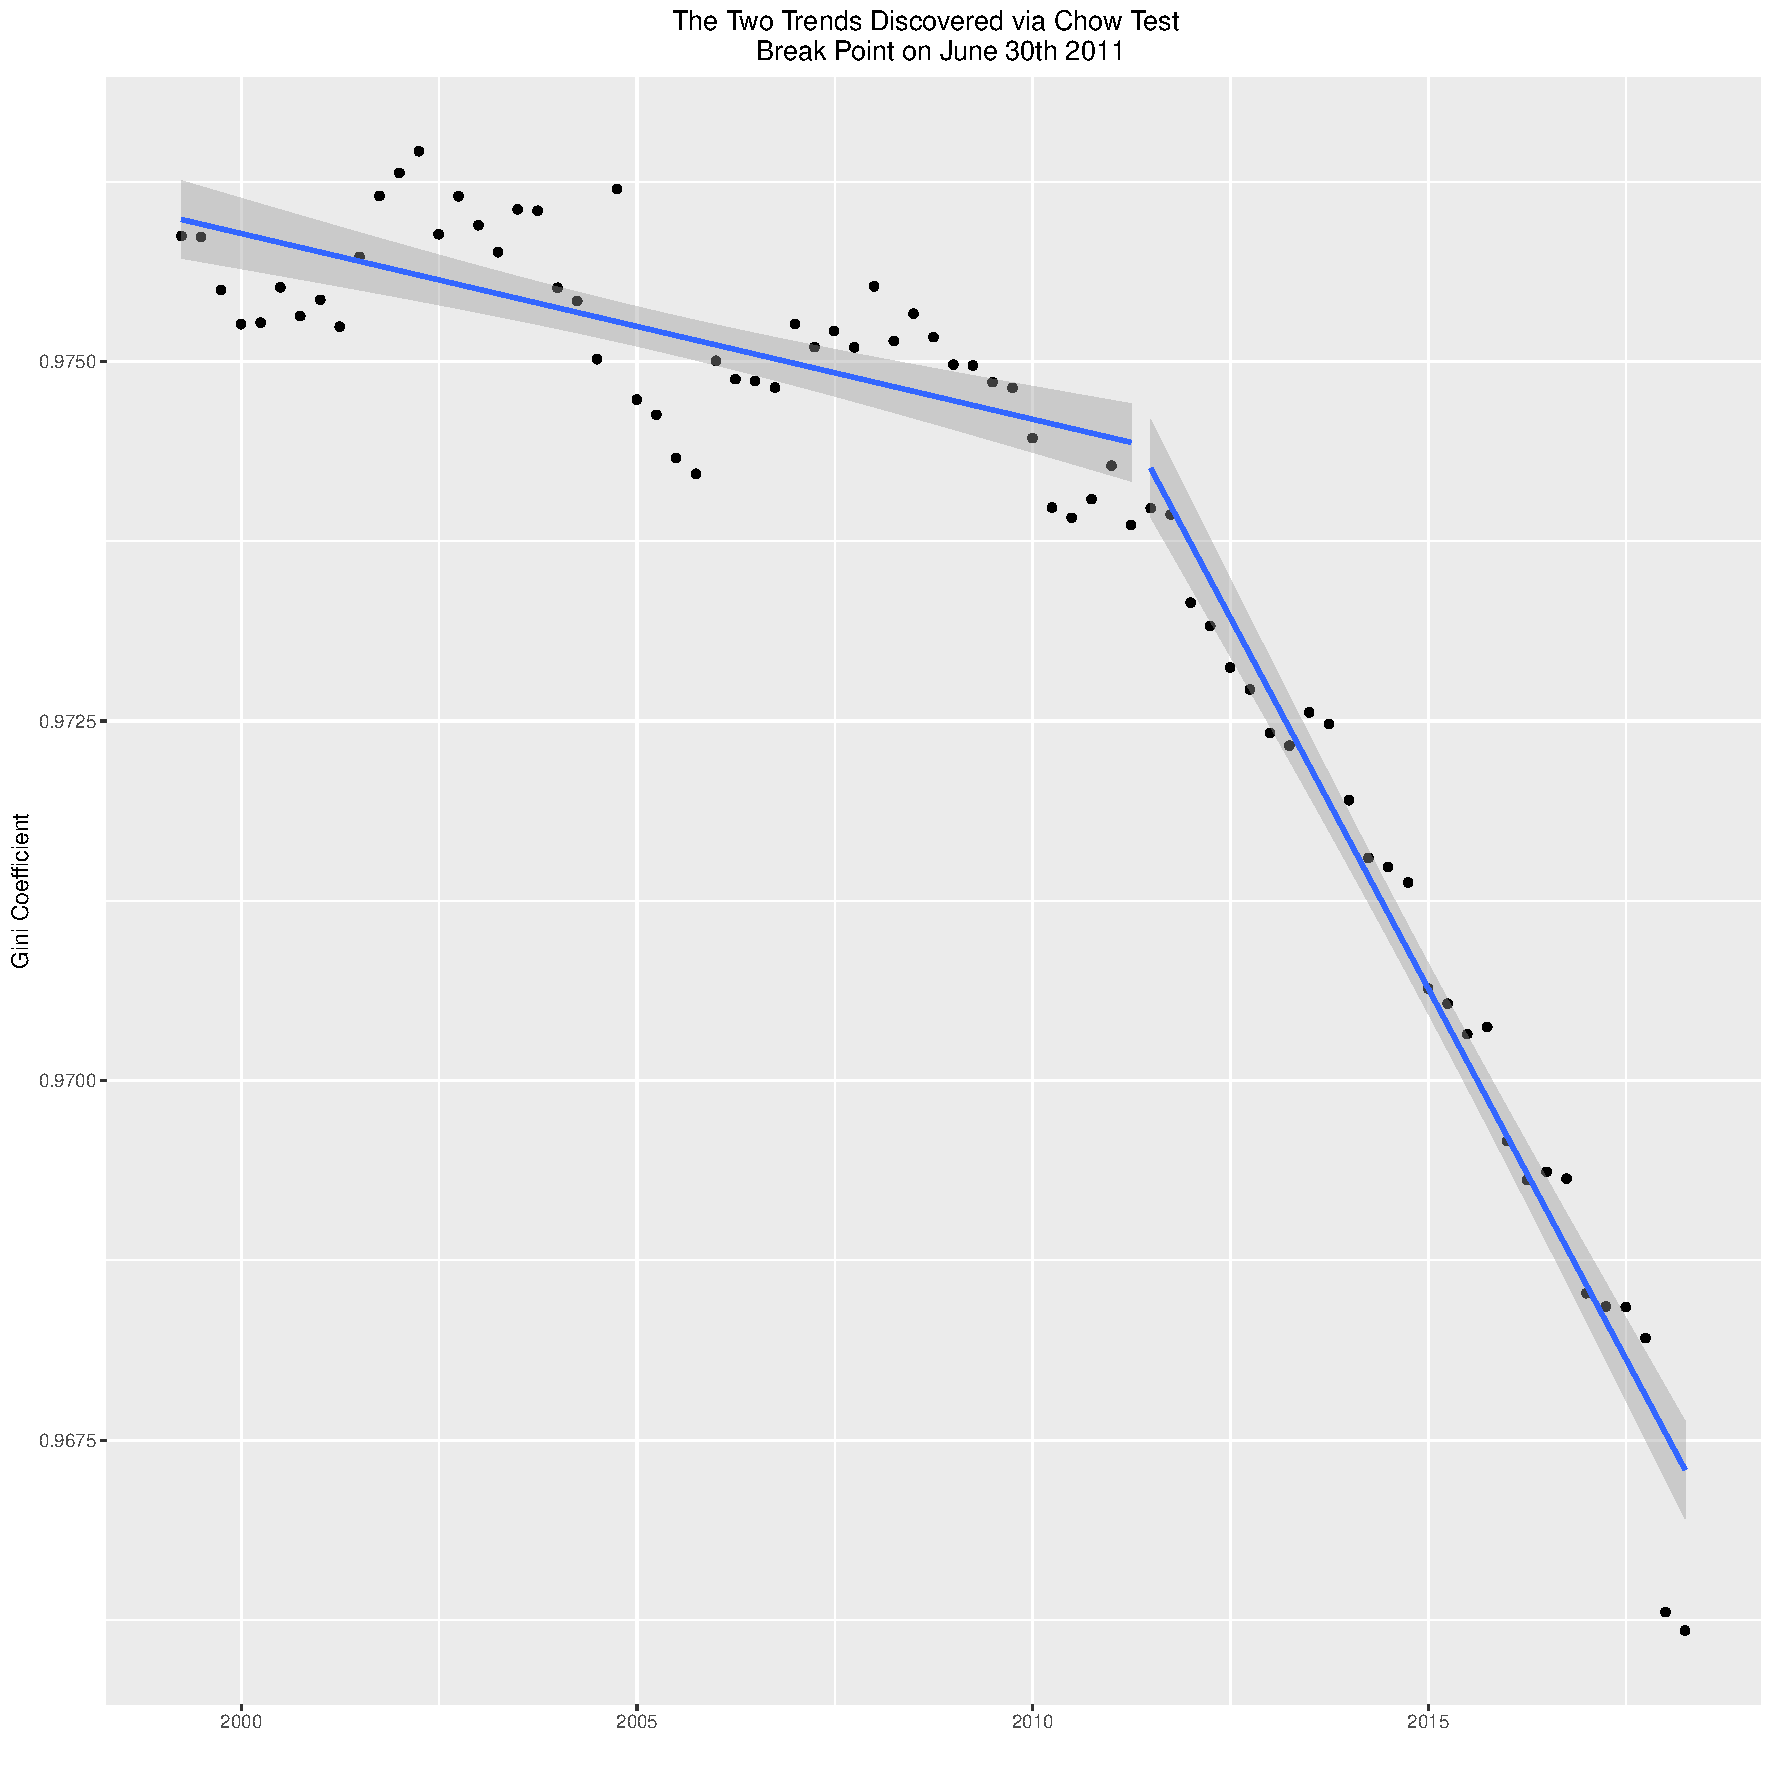
\includegraphics[width=1\textwidth]{Figures/ChapterIII/ChowTest.pdf}
	\caption[Chow Test Result]{Result of Chow test.  Breakpoint on June 30th 2011}
	\label{fig:Chow Test}
\end{figure}

\subsection{Investors by County Urban Intensity Index}

Counties (and their equivalents) are important building blocks in the American territorial administration.  However, not all counties are created equal.  For example, Los Angeles County in California has a population approaching 10 million people, whereas rural counties such as Loving County in Texas contains less than 200 inhabitants \citep{USCensus13}.  In the field of health geography and epidemiology, rural-urban divide can play a role in predicting health outcomes.  The National Center for Health Statistics devised a classification scheme for all US counties that can be used as a proxy for the degree of urban surface area in each county \citep{national2014urban}. This classifies counties into one of 6 different categories.
\begin{enumerate}
	\item Metropolitan Categories:
	\begin{enumerate}
		\item \textbf{Large Central Metropolitan counties} (Category 1) are counties in Metropolitan Statistical Areas (MSAs) with at least 1 million inhabitants, and one of the following characteristics: 
		\begin{enumerate}
			\item contain the entire population of the largest principal city of the MSA, or 
			\item are completely contained within the largest principal city of the MSA, or 
			\item contain at least 250,000 residents of any principal city in the MSA.
		\end{enumerate}
		Examples: New York County New York\footnote{Coterminous with Manhattan Borough in the City of New York}, Bronx County New York, Los Angeles County California, Cook County Illinois. 
		
		\item  \textbf{Large peripheral metro counties} (Category 2) are counties in a MSA with a population greater than or equal to 1 million, but do not qualify as category 1 county.  
		
		Examples: Orange County New York, San Mateo County California
		
		
		\item \textbf{Medium metro counties} (Category 3) are counties in MSA with a population greater than 250,000 but less than one million in population.
		
		Example: Fresno County California, New London County Connecticut
		
		\item \textbf{Small metro counties} (Category 4) are counties in MSAs with populations greater than 50,000 but less than 250,000 in population.
		
		Example: Yuma County Arizona, Franklin County Vermont
		
	\end{enumerate}
	\item	Non-metropolitan Categories:
	\begin{enumerate}
		\item \textbf{Micropolitan counties} (Category 5) are counties in a micropolitan statistical area
		
		Example:  Juneau City and Borough Alaska, Talladega County Alabama
		
		\item \textbf{Noncore counties} (Category 6) are counties that do not contain a micropolitan statistical areas
		
		Example: Loving County Texas, Denali Borough Alaska
	\end{enumerate}
\end{enumerate}


This categorisation of counties gives insight into the type of region the new institutional investors prefer. As predicted by Quaternary Location Theory, it is hardly surprising that institutional investors are primarily found in large urban areas. This was also hinted in Figures \ref{fig:countbycbsalegal},  \ref{fig:percentageofinvestmentfirmsbycbsa}, and \ref{fig:percentageoffirmsbycbsa}, where it shows that the majority of investors are clustered around the topmost cities in the American urban hierarchy.  Therefore, it should be of no surprise that Figure \ref{fig:changeinrelativenumberruralurban} indicates that 95 percent of institutional investors are located in Metropolitan counties, and that the share of investors in Micropolitan counties is quite stable over time.  The largest change is that category 2 counties see an increase in market share, which mostly comes at the expense of category 1 counties. This provides evidence that while downtown areas are slightly less attractive to investors, going for bargain basement land costs is also not a preferred strategy, or else we would see an uptick over time in the counts of category 5 or category 6 counties.  While the relative gains of category 2 counties are impressive, one should not lose sight of the fact that the largest absolute growth in the number of institutional investors occurs in category 1 counties (Figure \ref{fig:changeinabsolutenumberruralurban}).     

It should be noted that the drop in number of firms in the aftermath of the 2008 great financial crisis is of nearly equal proportion in all categories of counties (Figure \ref{fig:changeinrelativenumberruralurban}).  Yet it is quite evident when looking in absolute numbers of extant institutional investors (Figure \ref{fig:changeinabsolutenumberruralurban}) that category 1 counties take a longer period of time to reestablish their number of investors.  

This growth in secondary counties in a conurbation may also hint a second phenomenon, such as an increase preference and/or availability of suburban office space in response to the expense of downtown offices.  \cite{Pohl2004} examines the remaining stock of real-estate in Manhattan after the terrorist attack on the World Trade Center and concludes that the destruction of World Trade Center Buildings 1, 2 and 7, as well as the damage on the other buildings essentially removed nearly a quarter of Manhattan's tier 1 and 2 office space from the market, and that the resulting scramble for office space tightened Manhattans' office market, spilling over into the other 4 boroughs as well as suburban New York, New Jersey, and Connecticut.  



\begin{figure}
	\centering
	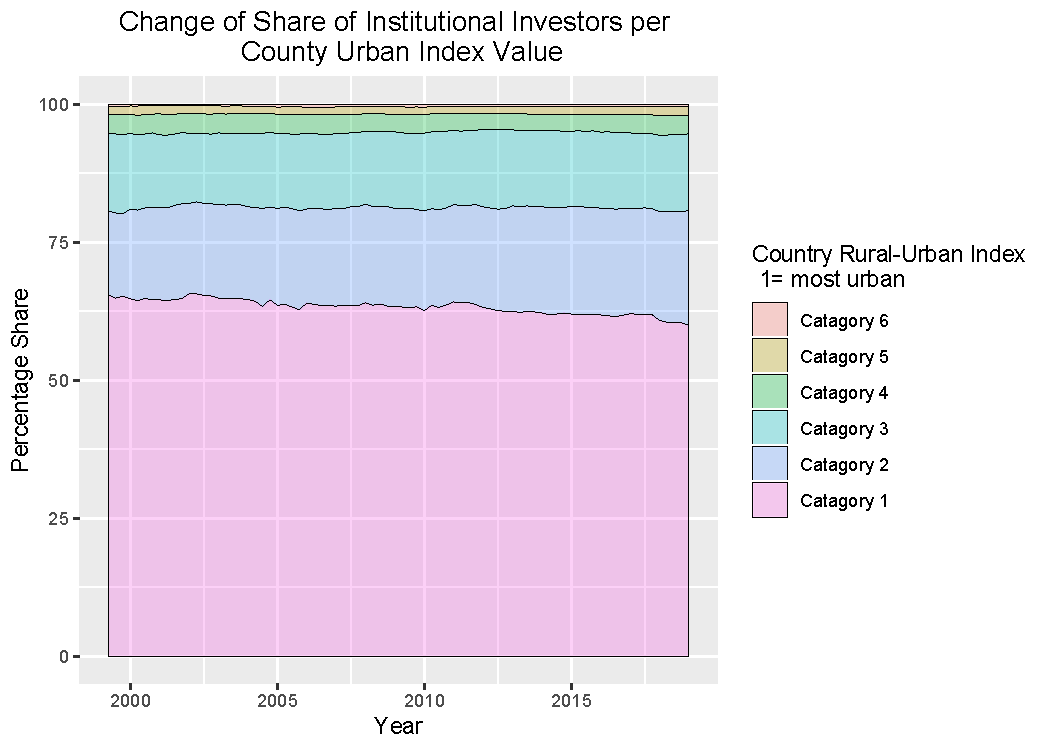
\includegraphics[width=1\linewidth]{Figures/ChapterIII/ChangeInRelativeNumberRuralUrban}
	\caption[Relative Numbers of Institutional Investors Over Time by County Urban-Rural Index]{Percentage share of firms by County Urban Index Value from 1999 to 2018}
	\label{fig:changeinrelativenumberruralurban}
\end{figure}

\begin{figure}
	\centering
	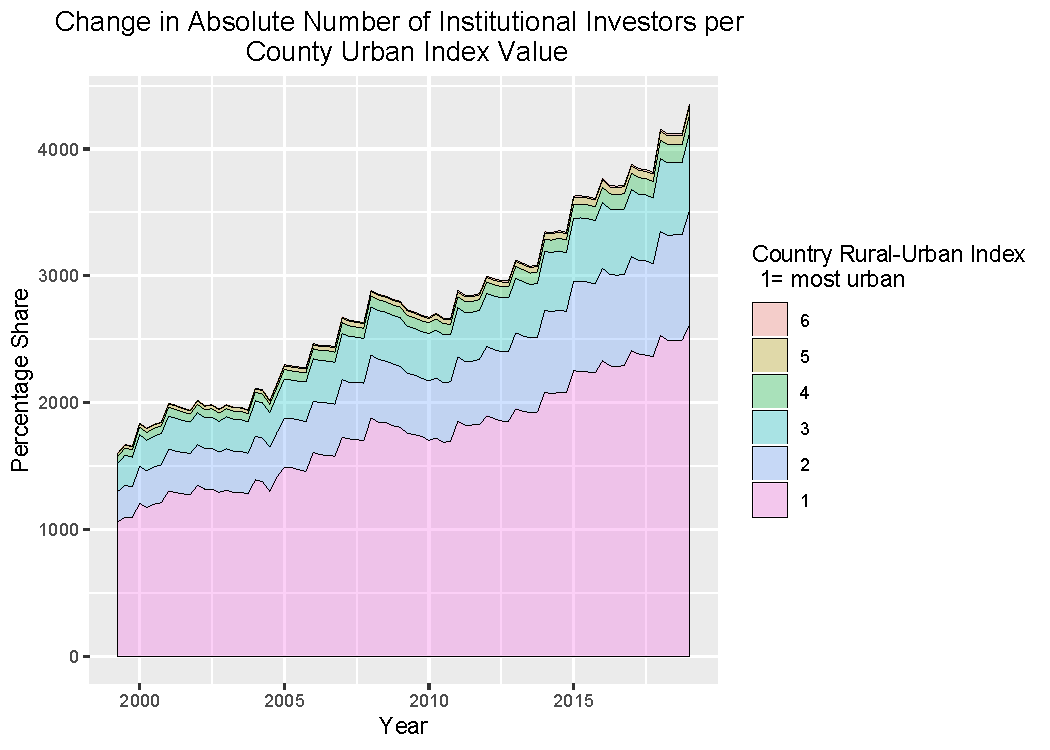
\includegraphics[width=1\linewidth]{Figures/ChapterIII/ChangeInAbsoluteNumberRuralUrban}
	\caption[Absolute Numbers of Institutional Investors Over Time by County Urban-Rural Index]{Count of firms by County Urban Index Value from 1999 to 2018}
	\label{fig:changeinabsolutenumberruralurban}
\end{figure}


\subsection{Investors By Region}

A way to reconcile the decline in market share of the New York region in Figures \ref{fig:precentagestate}, \ref{fig:percentageofinvestmentfirmsbycbsa}, and \ref{fig:percentageoffirmsbycbsa}  with Figures \ref{fig:changeinrelativenumberruralurban} and \ref{fig:changeinabsolutenumberruralurban} is to ask if the traditional definition of State or CBSA is too narrow, and that the declines may be partially explained by the modifiable area problem (MAP). \nomenclature{MAP}{Modifiable Areal Problem} The MAP is a source of statistical bias in geography-based data aggregation, since boundaries on reporting areas can have an outsized influence \citep{Fotheringham1991}.  A common extreme case of the MAP is gerrymandering, in which a political party can gain more seats relative to its vote share by controlling how the votes are aggregated into different districts.  In this case, all of the levels of aggregation seen so far (State, CBSA and County) fail to holistically capture Megaregions in the USA, and in particular the Boston-New York-Washington (Bos-Ny-Wash) megaregion  \citep{lang2007america}. While it may not fully encompass the Bos-Ny-Wash, the US Census Bureau's Region\footnote{\url{https://www2.census.gov/geo/pdfs/maps-data/maps/reference/us_regdiv.pdf} for a map listing the geographies encompassed by the different regions} does a good approximation of this.  

\label{Atlanta}

\nomenclature{Bos-Ny-Wash}{Boston-New York-Washington DC Megaregion}

In the case of Figure \ref{fig:Percentage_firms_Region_USA}, the decline of the North East is much slower than one would expect from previous graphs, mostly due to the inclusion of the south shore of Connecticut and the North shore of New Jersey.  


Increases in the number of Southern-based investors lies mainly in the growth of firms located in the DC/Arlington Virginia region as well as Atlanta. With regards to the decline of the Mid-West, as mentioned previously, this is more of a relative decline than an absolute decline, for while it started the study period with 321 (20\%) institutional investors and ended with 728 (17.6\%).


\begin{figure}
	\centering
	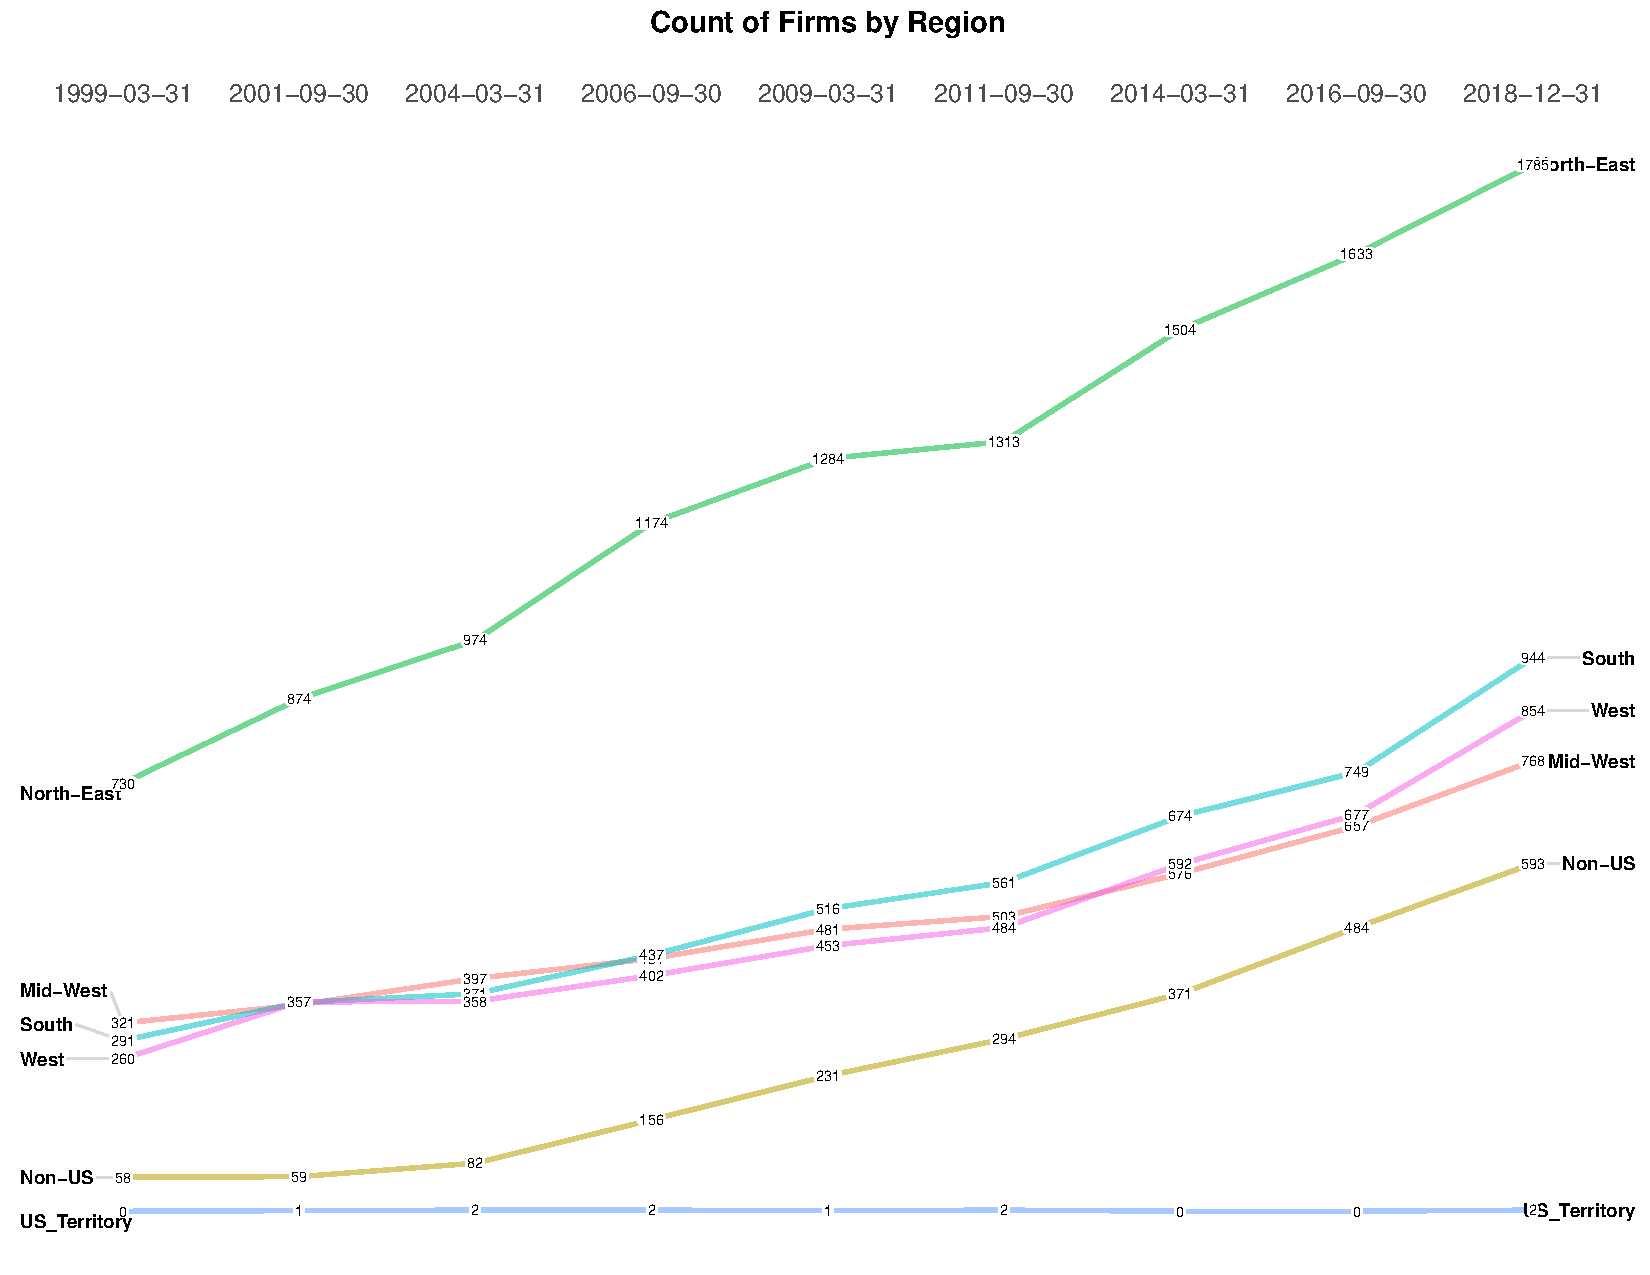
\includegraphics[width=1\linewidth]{Figures/ChapterIII/Count_firms_USA}
	\caption[Count of Institutional Investors by Region (as defined by the US Census Bureau) for the Period 1999 to 2018]{Relative percentage of institutional investors by region during the study period (March 1999 to December 2018)}
	\label{fig:countfirmsusa}
\end{figure}

\begin{figure}
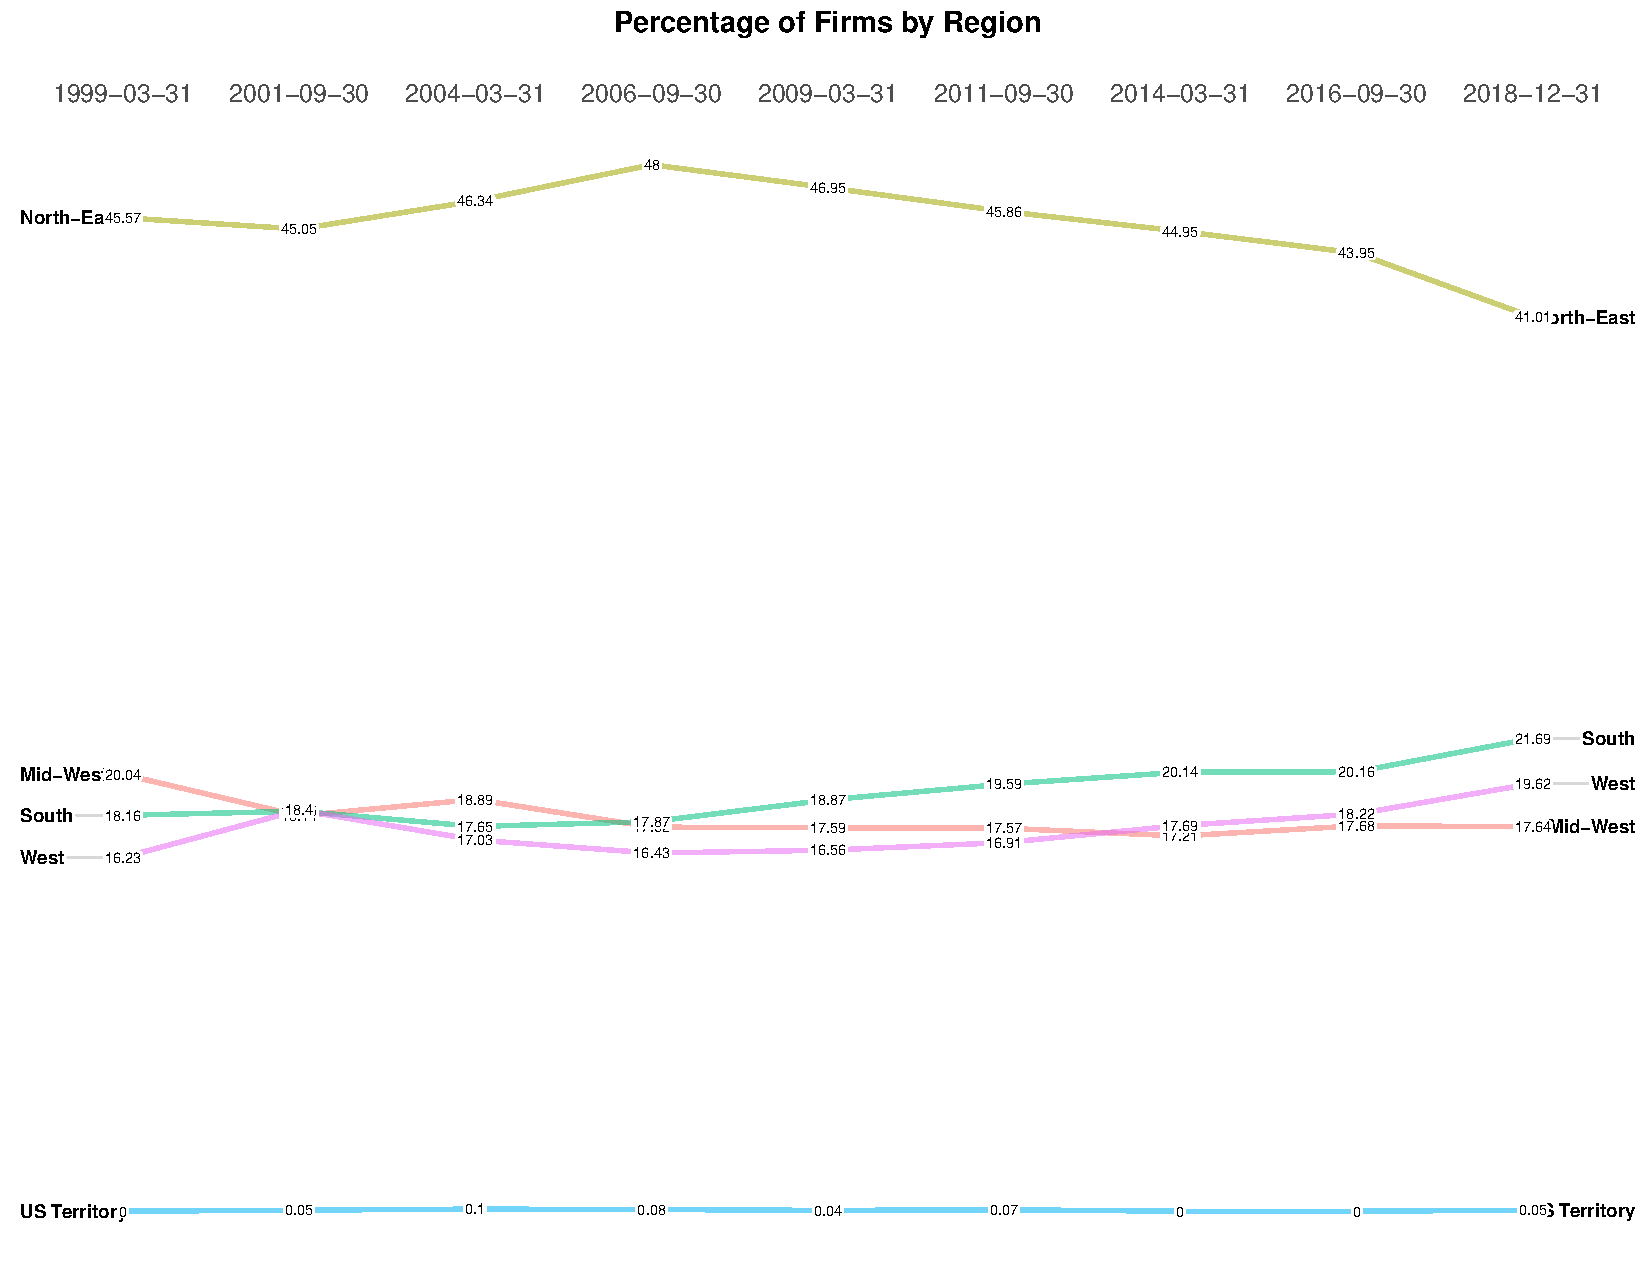
\includegraphics[width=1\linewidth]{Figures/ChapterIII/Percentage_firms_Region_USA}
\caption{Number of Firms by US Region}[Total number of firms by region  (as defined by the US Census Bureau) during the study period (March 1999 to December 2018)]
	\label{fig:Percentage_firms_Region_USA}
\end{figure}

%\subsection{Distances}

%distances calculated with the geosphere package citep{geosphere}

\section{The K-function} 
\label{kfunction}
One of the earliest uses of point pattern analysis is the famous cholera map by Dr. John Snow.  Although he knew nothing about the cause of the bacterial outbreak, he did discover that the cases of cholera were clustered around a particular water pump on Broad Street.  Although scholarship such as \cite{brody2000map} call into question whether Dr. Snow's map was more confirmatory than exploratory since the insights into the cause of the cholera epidemic requires an understanding of germ theory.  That is to say, that these maps would not be able to create their historic insights without subject matter expertise.  Regardless of whether Dr. Snow used his point density mapping technique as a starting point or only for confirmation of his hypothesis,  a common method of quantifying points in space is measuring the intensity of the point pattern per unit of area.  Old staples used for measuring point patterns are quadrat analysis and nearest neighbour index.  However, these techniques have well known limitations such as the undue influence caused by border selection as well as the inability to determine whether points cluster or disperse at different ground scales \citep{spatstatBook}.

The examination of various ground scales is important since firms may exhibit different clustering tendencies at various scales.  The mirroring of population maps and geographic profile maps at a national scale is humorously examined in XKCD comic 1138 (Figure \ref{fig:heatmapxkcd}) \citep{XKCD1138}.  However, firms may behave differently at different scales.  For example, a national maps of firms such as coffee shops, fast food chains, banks, automated teller machines, gas stations and grocery stores may mirror the national population map, yet they would appear diffuse on a local map, for each operates their own local catchment areas.  However, other sectors such as software development have a tendency to cluster at the local and regional level \citep{Meyer2006}.  

\begin{figure}
	\centering
	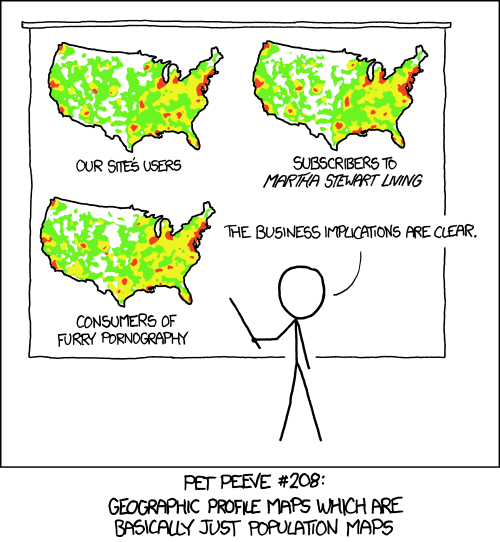
\includegraphics[width=0.5\linewidth]{Figures/ChapterIII/heatmap_XKCD}
	\caption[XKCD 1138 - Heatmaps]{XKCD \#1138 - Heatmaps by Randall Monroe. This illustrates the point that many patterns can be approximated by human density. Used with Permission (Creative Commons Attribution-NonCommercial 2.5 License)}
	\label{fig:heatmapxkcd}
\end{figure}

At its most basic form, the K-function calculates using a Poisson process of actual verses expected counts of points within distance $h$ of each point in the data set \citep{dixon2014r}.  This yields a density function which can be compared to the expected point pattern intensity under the conditions of complete spatial randomness at different distances.  For more information about\textit{ Ripley's K}, see \cite{ripley1976second,fischer2009handbook,spatstatBook}.

With regards to examining the clustering behaviour of institutional investors at various scales, the inherent ability to be used at various ground scales makes Ripley's K well suited for examining the clustering behaviour of institutional investors.  This facilitates the examination  of spatial clustering of institutional investors  and determines if they exhibit locational preferences closer to that of ATMs or software developers. 

The K-function in it's most basic form can be written as follows:  

\begin{equation}
K(d) = \lambda^{-1}E(Nd)
\end{equation}
Where $Nd$ is the number of events $Xi$ within distance $d$ of a randomly chosen event from all points $\{X_{i},...,X_{j} \}$.  When working with a sample of data points $\{ X_{j} \}$, the K-function for the underlying distribution isn't usually known.  However, it can be estimated by using a sample.  If $d_{ij}$ \todo{finish this} 

\begin{equation}
\hat{K}(d) = \hat{\lambda}^{-1}\sum_{i}\sum_{i \neq j}\dfrac{(d_{ij} < d)}{n(n-1)}
\end{equation}

\begin{equation}
    \hat{\lambda} = \dfrac{n}{|A|}
\end{equation}

The CSR equation
\begin{equation}
    K_{csr}(d) = \pi d^{2}
    \label{eq:csr}
\end{equation}

Where $|A|$ is the surface area of the study.  In order to determine whether a sample is clustered or dispersed, one compares $K_{CSR}(d)$ to $\hat{K}(d)$.  If the generated sample is sufficiently different than what one would expect under CSR, one may conclude that the underlying process generating the events is not influenced by a random spatial process \citep{brunsdon2015introduction}. 

\subsection{Spherical K-function}

The basic implementation of \textit{Ripley's K} technique assumes that the point pattern exists on a Euclidean surface.  While it may be justifiable to assume a Euclidean plain for regions of less than a few hundred kilometres \citep{HeatherJ.Lynch2008,wilschut2015spatial},  the use of Euclidean space becomes problematic above such distances, and the global distribution of institutional investors is certainly more than a few hundred kilometers, and thus spherical geometry becomes a better option. Furthermore, \cite{Tobler2002} demonstrates that while the Earth is technically an oblate spheroid, most statistical techniques on a continental scale can be done adequately on a sphere.  

The K-function displayed in Figures \ref{fig:Kfunction1}, \ref{fig:Kfunction5to100}, \ref{fig:Kfunction100to750}, and \ref{fig:Kfunction1000to5000} were performed in statistical language R using Robeson's implementation of spherical geometry on Ripley's K \citep{SphericalK}.  This analysis was conducted with a 99-fold cross-validation, in which for each time step, the 1/99 of the data was randomly reserved from the data set\footnote{The calculation of the K function for the 80 quarters involved in this study was performed on 3 different computers for a duration of 3 months for a total of 9-computer/months calculation time}.  This creates an envelope of possible K-functions. Particular care should be noted for the third and fourth quarters of 2004.  These quarters were run a second time with a similar result, suggesting that the problem may lie with the data pipeline from Edgar rather than a sudden and reversible shift in locations preference. A similar, but less extreme discontinuity exists between the fourth quarter of 2013 and the first quarter of 2014. 

As with the other forms of measuring the concentration and dispersion at various scales seen earlier, the overall trend of initial concentration and dispersion on or after 2007 continues with the K-function.  In greater detail, Figure \ref{fig:Kfunction1} looks at the 1 km scale, where there is an initial concentration followed by a gradual diffusion starting on or around 2003. Figure \ref{fig:Kfunction5to100} shows a slightly different picture, more akin to the County and CBSA graphs of concentration from 1999 to on or about 2007 and an increased diffusion afterwards.  Figure \ref{fig:Kfunction100to750} shows a similar pattern - just not as starkly.  Finally, Figure \ref{fig:Kfunction1000to5000} shows that the continental scales resemble the shape seen in Figure \ref{fig:Kfunction1}, since there is a continual diffusion of firms from a earlier peak.  

This is an important confirmation of the trend, since Ripley's K is a point pattern analysis, and is thus immune to the  modifiable areal unit problem.  This suggests that something fundamental in the business world occurred in the time-frame of the pivot that changed the calculus in terms of benefits of the forces of agglomeration and desegregation.  There is precedence in the location preferences shifting in the past, with a substantial amount of dispersion occurring in the 1970s and 1980s when the first telecommunication revolution occurred \citep{bodenmanfirm2000}.

While it is beyond the scope of this research, it would be interesting to examine if the rise of so called business-oriented ``smartphones" by Blackberry (formerly known as Research In Motion), touchscreen smartphones such as ``iPhone" and ``Android" devices, in addition to widespread wifi-enabled cafes have reduced the productivity tax of conducting business away from the office, and thus reduce the costs of locating outside of the central business district.   

\begin{figure}[h]
	\centering
	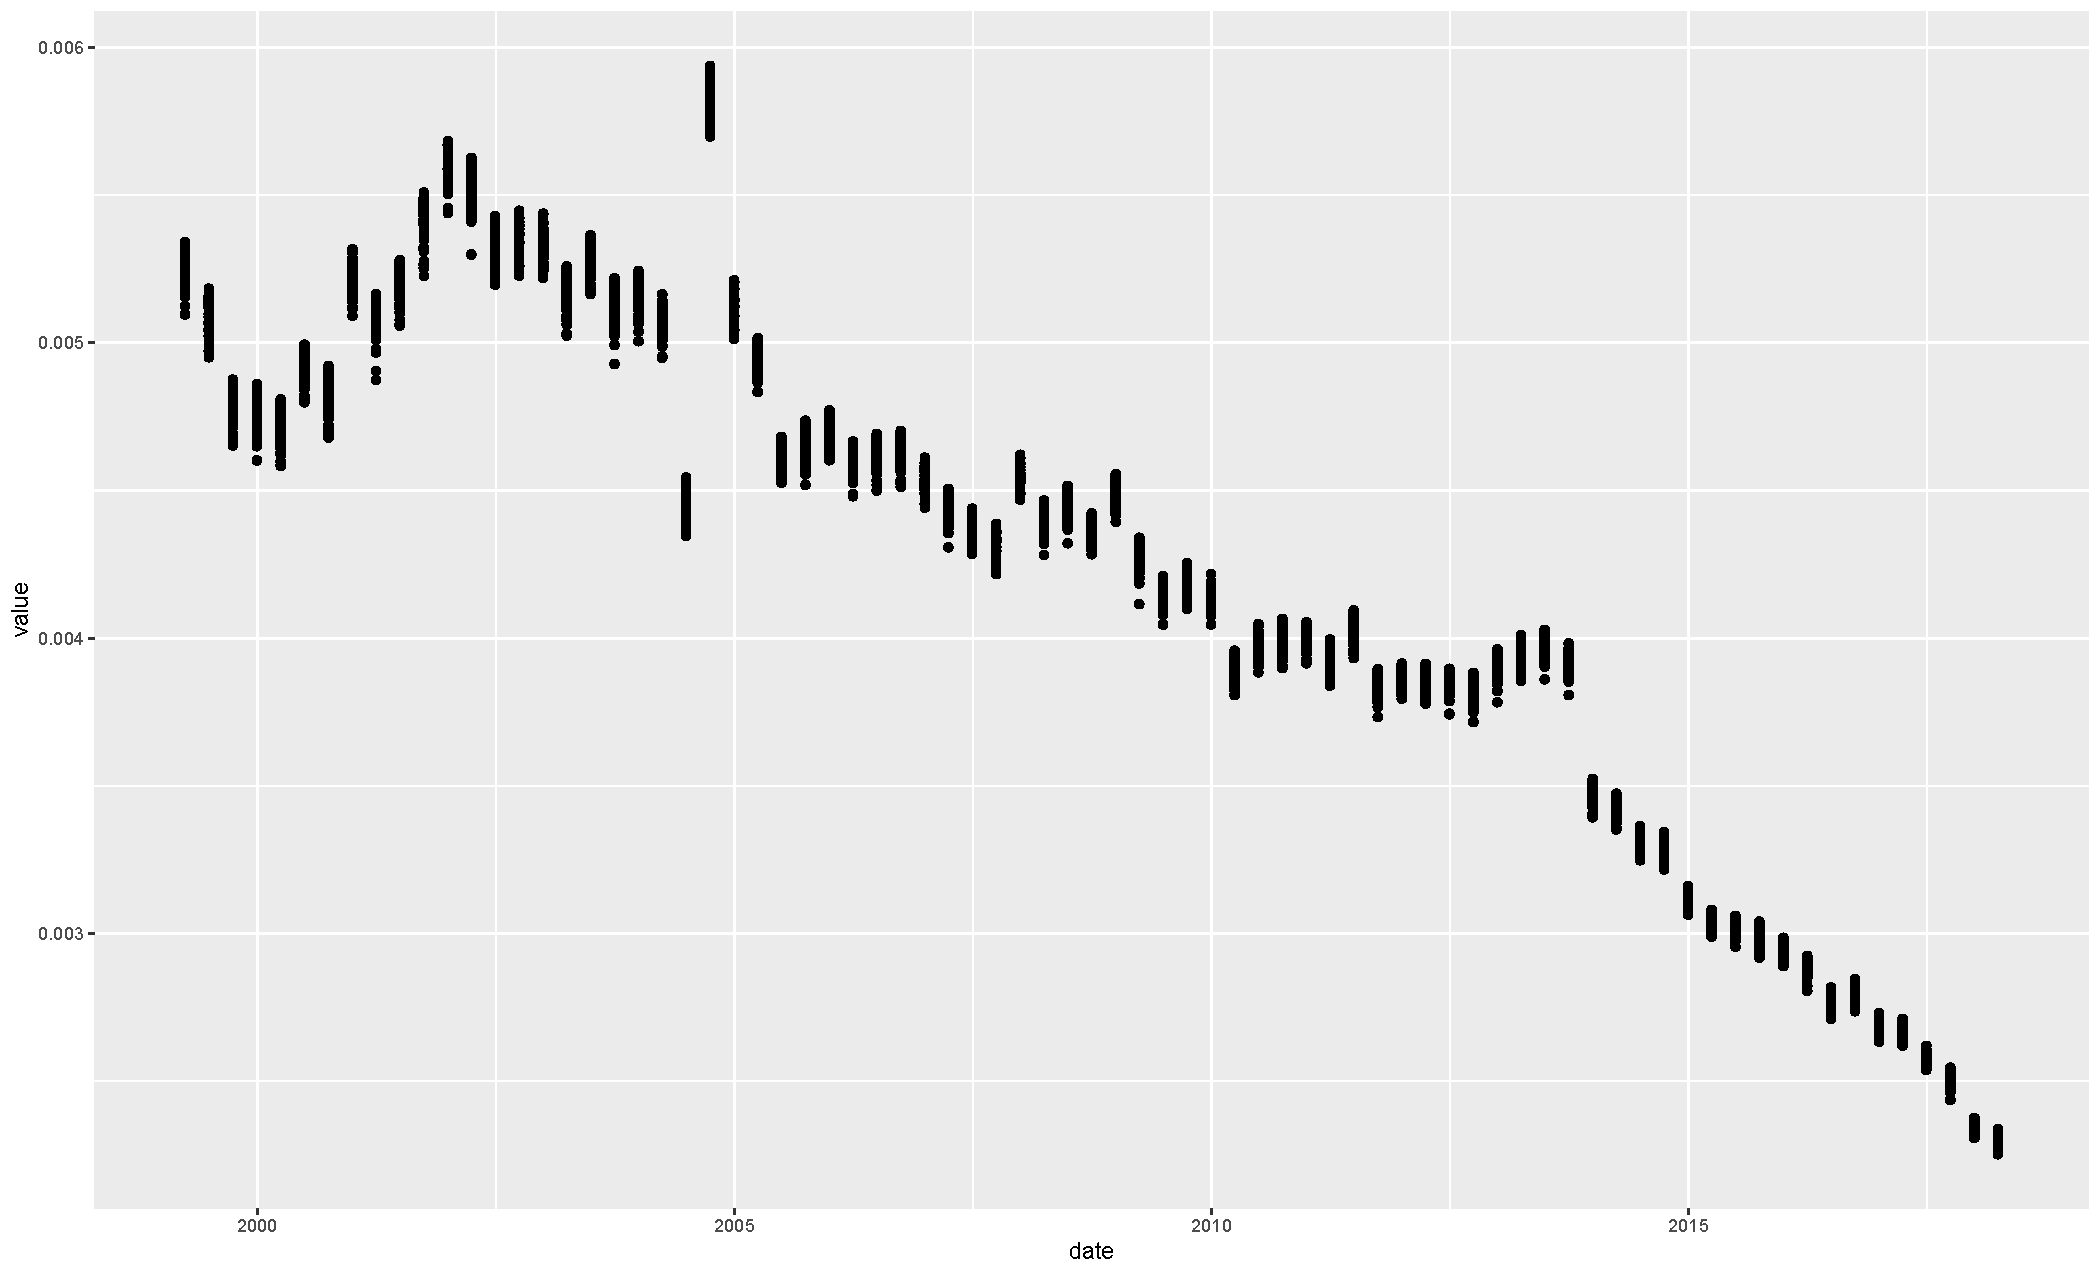
\includegraphics[width=1\textwidth]{Figures/ChapterIII/Cross_Val_1k.pdf} 
	\caption[Spherical K-function for Range Band 1km]{Spherical K-function for the range band of 1 km for the years 1999 to 2018.  Each quarter consist of 99 points representing a cross-validated K-function.}
	\label{fig:Kfunction1}
\end{figure}

\begin{figure}[h]
	\centering
	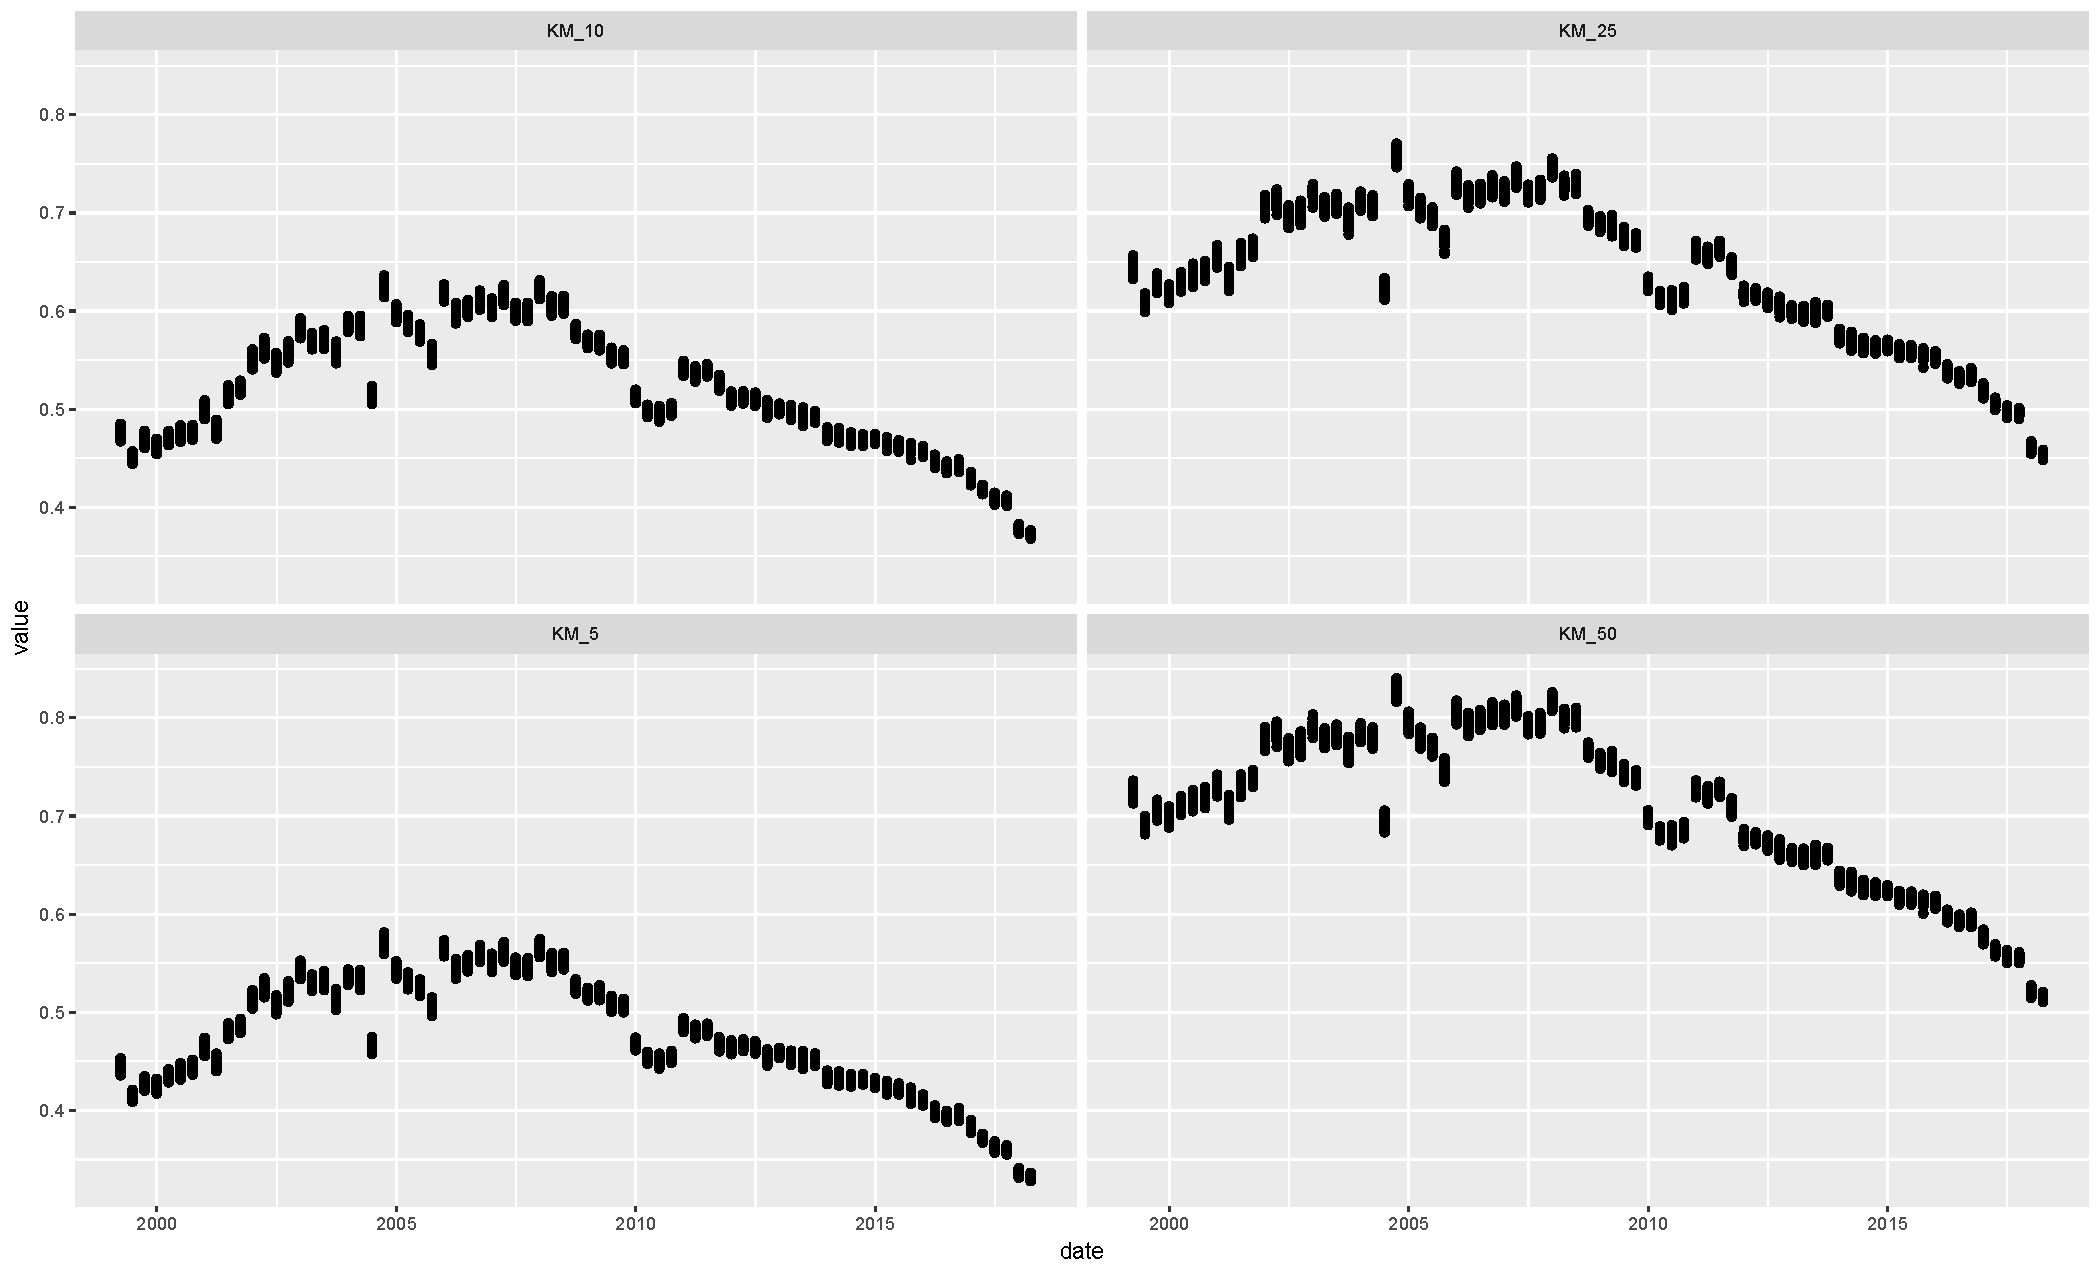
\includegraphics[width=1\textwidth]{Figures/ChapterIII/K_Function_5to50.pdf} 
	\caption[Spherical K-function for Range Bands 5km to 50km]{Spherical K-function for range bands 5km, 10km, 25km, 50km for the years 1999 to 2018. Each quarter consist of 99 points representing a cross-validated K-function}
	\label{fig:Kfunction5to100}
\end{figure}

\begin{figure}[h]
	\centering
	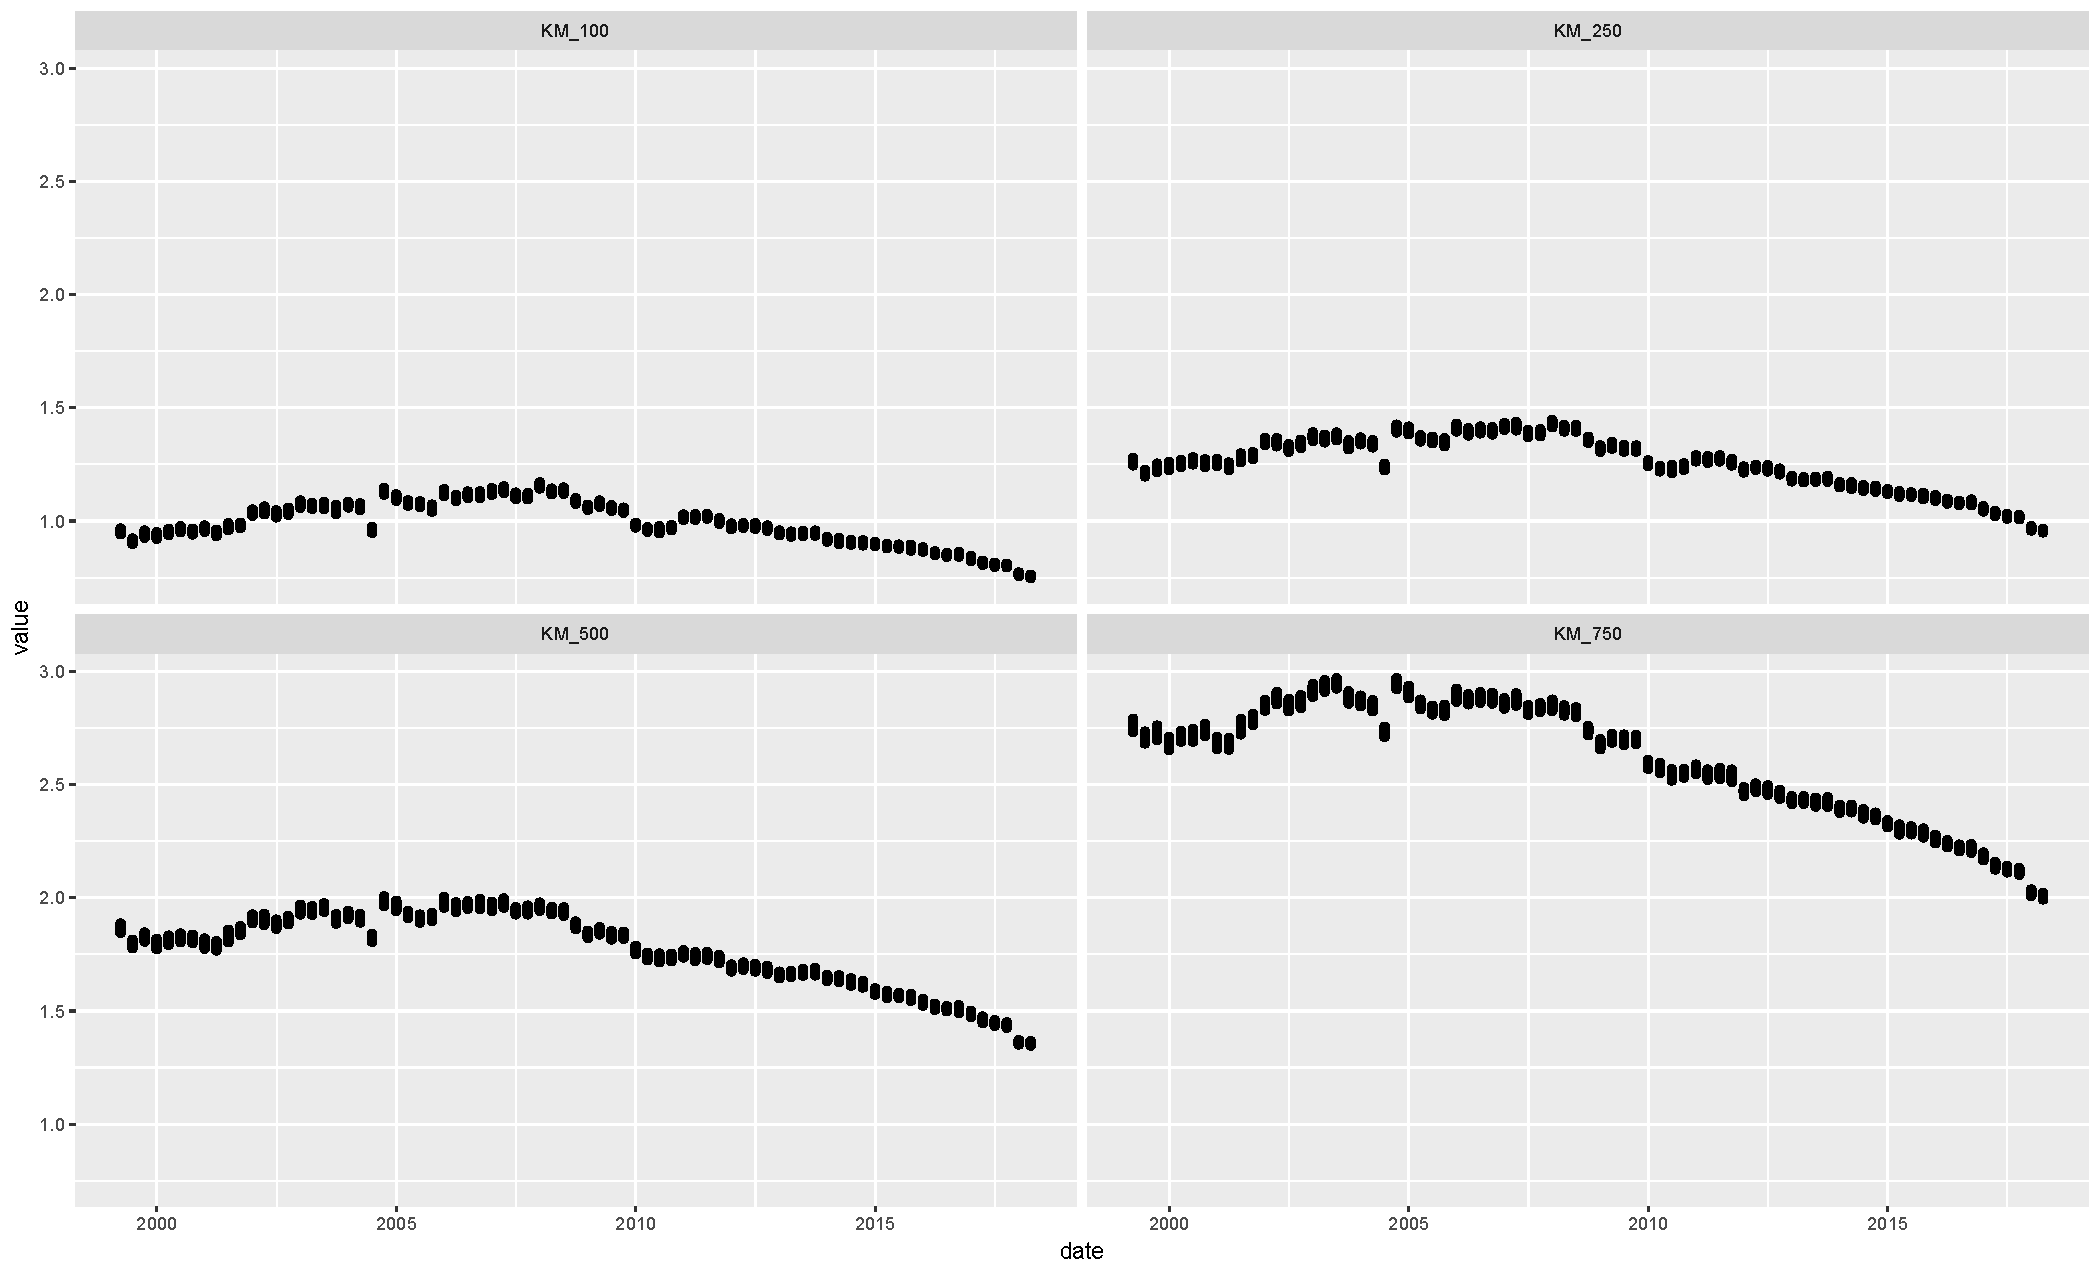
\includegraphics[width=1\textwidth]{Figures/ChapterIII/RIpley_K_100_750.pdf} 
	\caption[Spherical K-function for Range Bands 100km to 750km]{Spherical K-function for range bands 100 km, 250 km, 500 km, 750 km for the years 1999 to 2018. Each quarter consist of 99 points representing a cross-validated K-function}
	\label{fig:Kfunction100to750}
\end{figure}


\begin{figure}[h]
	\centering
	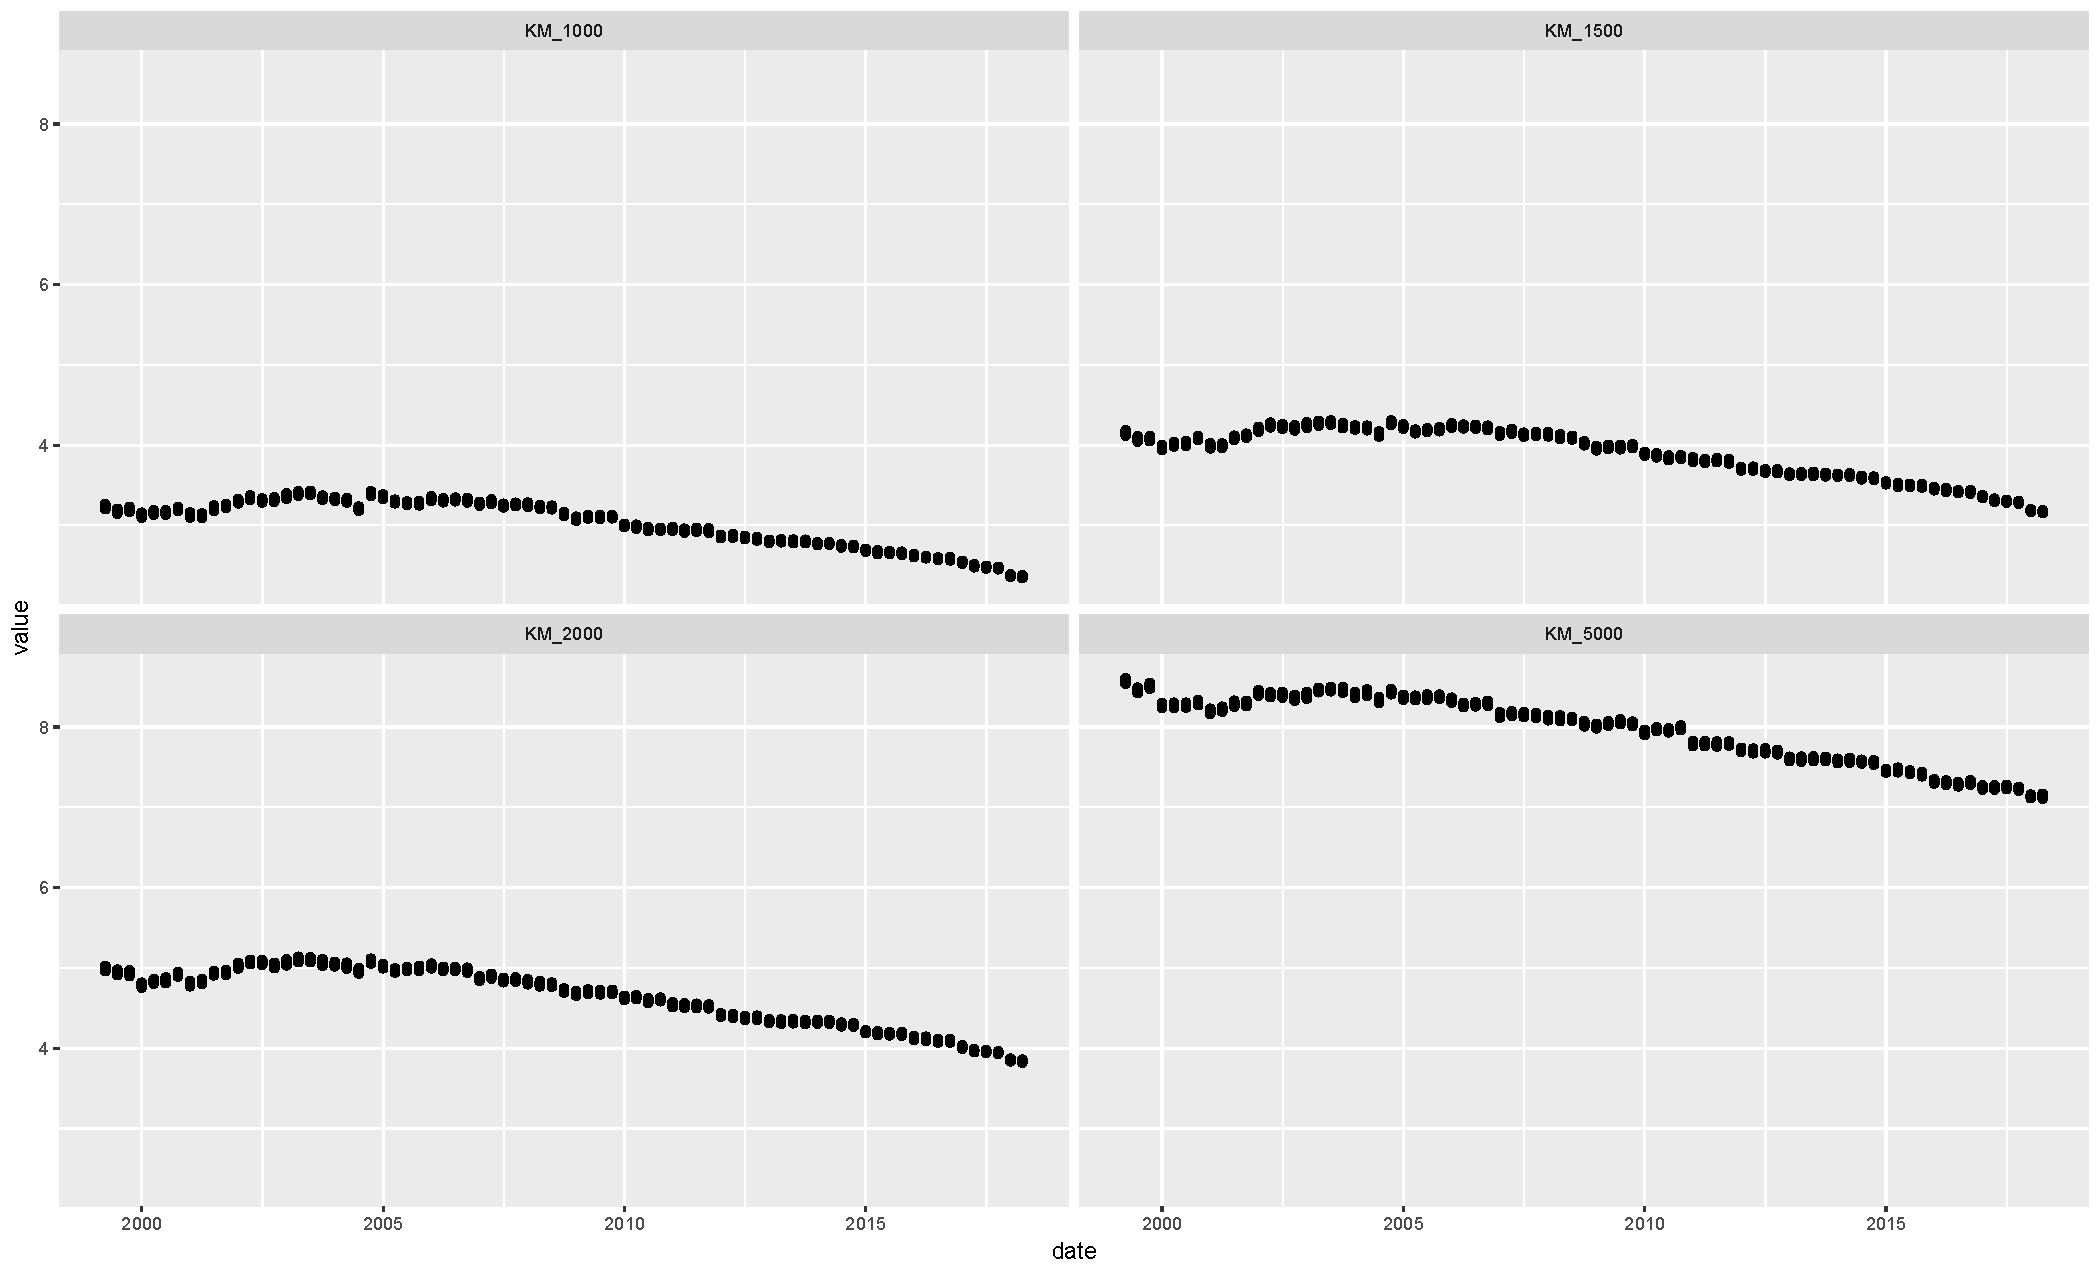
\includegraphics[width=1\textwidth]{Figures/ChapterIII/Cross_val_1000_5000.pdf} 
	\caption[Spherical K-function for Range Bands 1000km to 5000km]{Spherical K-function for range bands 1000 km, 1500 km, 2000 km, 5000 km for the years 1999 to 2018. Each quarter consist of 99 points representing a cross-validated K-function}
	\label{fig:Kfunction1000to5000}
\end{figure}





\section{Standard Deviation Ellipsis}

The standard deviation ellipse is a useful tool in measuring the dispersion of a point pattern, and comparing the same region at different points in time in order to draw insights about a particular phenomenon \citep{Yuill1971}. The standard deviation ellipse, and its simpler cousin the standard deviation circle, create a line that enclose one standard deviation of all points from the centre of all points.  The surface area contained by this line allows researchers to characterise the concentration or diffusion of a phenomena, and multiple such ellipses allow for the examining of a trend.  Figure \ref{fig:standarddeviationellipse} shows the evolution in time of the standard deviation ellipse for the five cities that contain the largest amount of institutional investors. As is consistent with the other measures of clustering examined so far, these 5 cities show a long-term trend towards diffusion as investors start to show up in suburban office parks. Furthermore, while it can be somewhat imprecise to directly compare densities across cities due to the vagaries of urban planning, it is almost impossible for Los Angeles County to appear denser or more concentrated in a particular metric than New York County (Manhattan). It is immediately apparent that Los Angeles' famous urban sprawl and lack of a proper CBD create a rather diffuse concentration of institutional investors - a point that will be visited in more detail in the following chapter.  

That being said, the advantage of the standard deviation ellipse over the standard deviation circle is the addition of orientation and eccentricity. Eccentricity is measured on a scale of 0 (perfect circle) to 1 (perfectly straight line).  An increase in eccentricity with a commensurate increase in surface area is suggestive of a new cluster being created near the perimeter of the ellipse. This is the case with regards to Boston in the mid-aughts in the Route 128 corridor (Figure \ref{fig:Standard_Deviation_ellipse_Eccentricity}). This will be examined in further detail Chapter \ref{subsection:Boston}.     

For the detailed metrics of the one standard deviation ellipse, see Appendices \ref{tab:Bos_SE} for Boston, \ref{tab:Chi_SE} for Chicago, \ref{tab:LA_SE} for Lost Angeles, \ref{tab:NY_SE} New York City and, \ref{tab:SF_SE} San Francisco.  

\begin{figure}
	\centering
	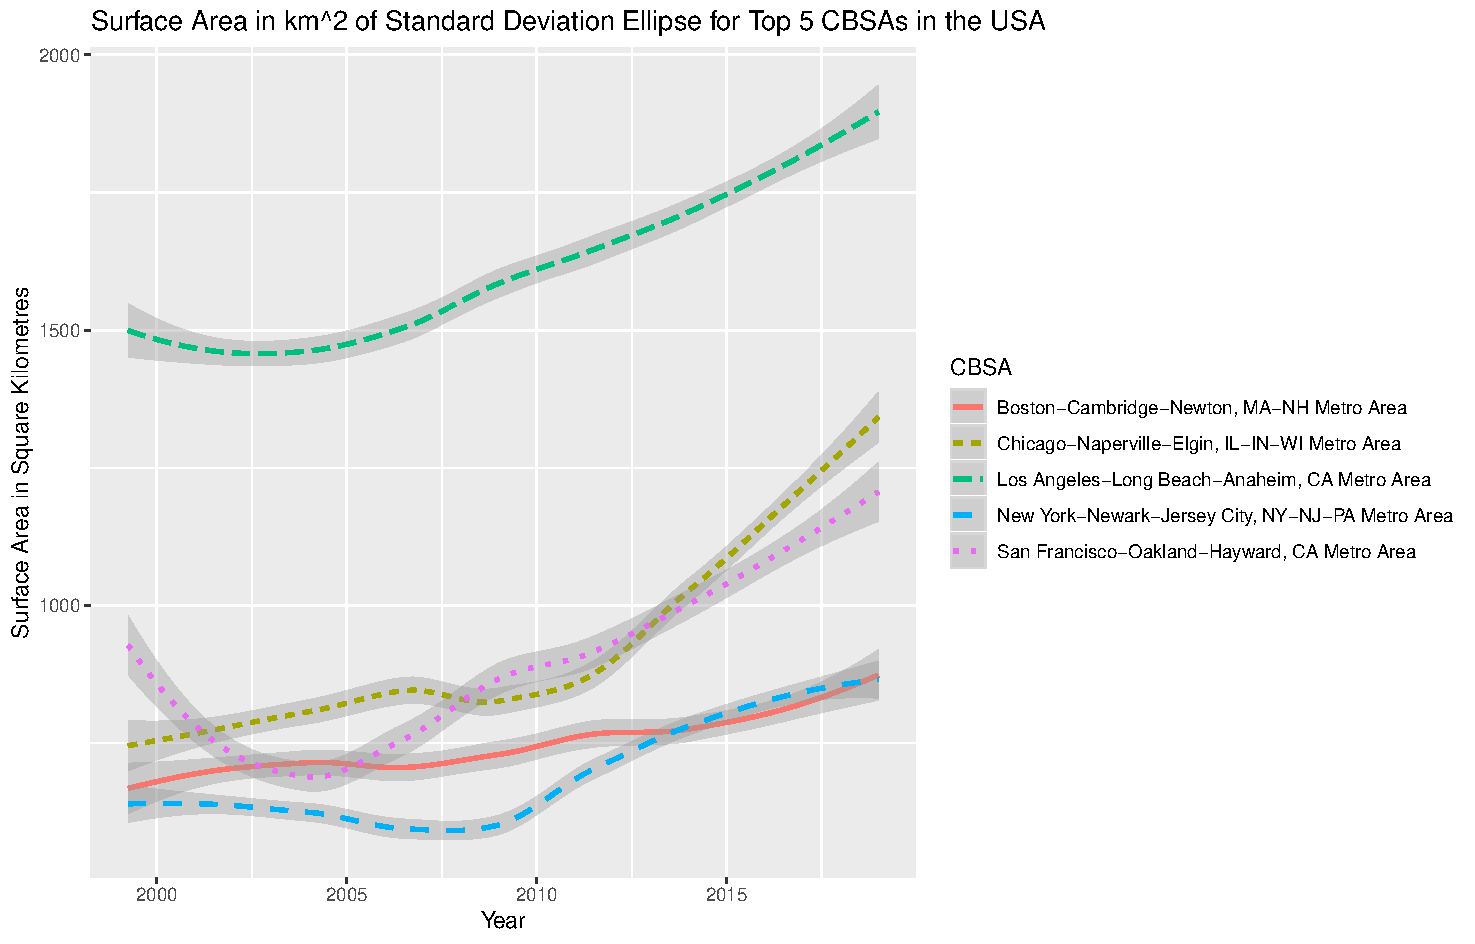
\includegraphics[width=1\linewidth]{Figures/ChapterIII/Standard_Deviation_ellipse}
	\caption[Standard Deviation Ellipse]{Standard deviation ellipse over time for the top 5 CBSAs by number of institutional investors for the time period of 1999 to 2018.}
	\label{fig:standarddeviationellipse}
\end{figure}

\begin{figure}
	\centering
	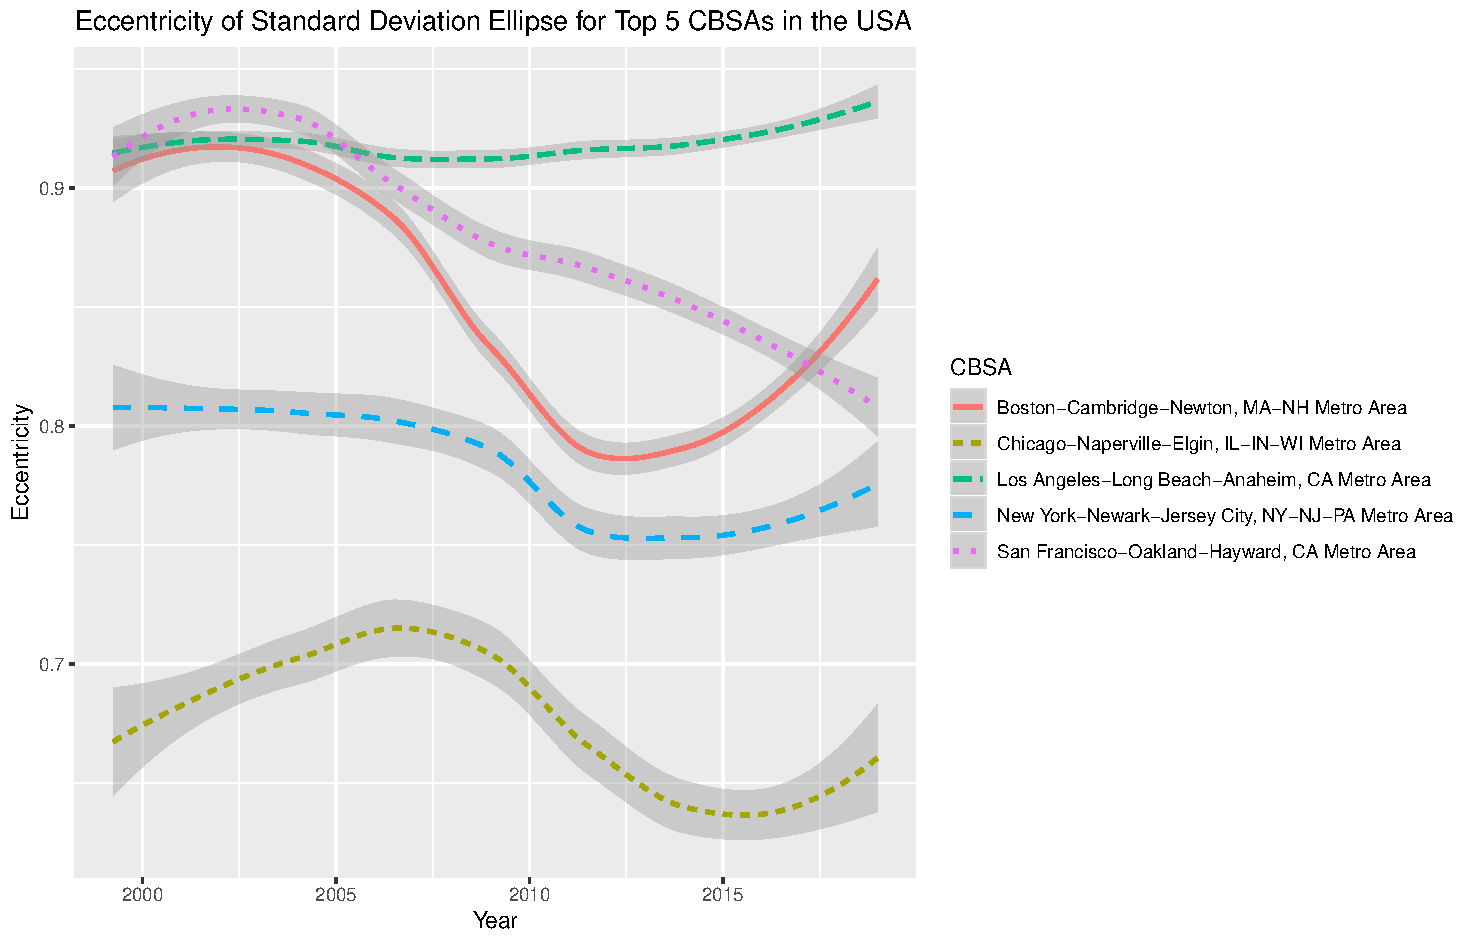
\includegraphics[width=1\linewidth]{Figures/ChapterIII/Standard_Deviation_ellipse_Eccentricity}
	\caption[Standard Deviation Ellipse Eccentricity]{Standard deviation ellipse eccentricity over time for the top 5 CBSAs by number of institutional investors for the time period of 1999 to 2018.}
	\label{fig:Standard_Deviation_ellipse_Eccentricity}
\end{figure}


\section{The Gravity Model of Trade}


Gravity model of trade is an empirically derived technique to describe and predict flows from a variety of origins to destinations.  One of the first researchers to propose a model for explaining flows of population across space is  \cite{ravenstein1885laws}. He identified a series of "laws" of migration, while not explicitly referencing Newtonian gravity, identified the key variables of distance as well as push and pull factors \citep{Tobler1995}.  

The most naive way of allocating flows across a land mass is to assume a uniform distribution.  However, this is questionable at best, for this disregards a myriad of variables that can be used to account for differences in trade.  Nobody would seriously expect that trade between New York County, New York (Manhattan) and Loving County, Texas to be on the same level as that between New York County, New York and Los Angeles County, California.  Standardizing the flow by a variable such as population might help, but there's no guarantee that the flow scales solely with population \citep{Crymble19}.   

The most naive version of the gravity model is as follows:
\begin{equation}
F = G \frac{M_{1}M_{2}}{r^{2}}
\label{Naive_Gravity_Model}
\end{equation}  

Equation \ref{Naive_Gravity_Model} is inspired by Sir Issac Newton's gravity equation.  As with the gravity equation, $F$ represent the trade in goods from points $M_{1}$ to $M_{2}$. $M_{1}$ and $M_{2}$ represents the aggregate push and pull factors and is traditionally measured as the size of each's market. $r^{2}$ is the square of the distance between these points and $G$ is a constant representing the friction of trade, such as the conditions of the roads, the productivity of the longshorepeople or tariff regimes.  Unlike the theoretical apple falling from a tree (or the spherical cow thrown by a frictionless trebuchet in a vacuum), human endeavours are plagued by free will and the myriad of uncertainty that follows.  However, in an insight that could have come from Isaac Asimov's Hari Seldon, populations are easier to model than individuals, since the vagaries of human existence averages out in the aggregate.  

A gravity model's goal is to tell the user: Given a number of influencing forces (distance, costs of living, desirability, access to services, access to markets) affecting the movements of a large number of entities of the same type (fungible commodities or similarly situated people) between a set number of points, what is the most probable distribution?  Furthermore, comparing real-world flows to the model's prediction can be used to find anomalies, and these can be useful starting points for future research\citep{Crymble19}.  

With respect to the gravity model, one must make sure that the data is either complete or a representative sample of the underlying flows, else the model will be hopelessly biased.  In this case, the model will be using the universe of 13F holdings for the period of June 2013 to December 2018 to create flows between investors and to the company in which the stocks belong.  The destination information is drawn from the COMPUSAT database \citep{Compustat} of stock information filings, and more specifically, the address of their headquarters which was subsequently geocoded using Google Maps.  The push and pull factors were calculated as the total stock ownership in the 13F database for each quarter in each CBSA.  CBSAs were used for this analysis rather than States ($n=50$) or counties and their equivalents($n=3,142$) due to the CBSA's occupation of a ``sweet spot'' with regards to detail and manageability  ($n= 935$, of which there are 465 CBSAs which contain at least one flow).  

\begin{table} 
	\begin{center}
	\small
		\caption[Gravity Model of Trade for Q2 2013]{Gravity model of trade as applied to investment flows between US CBSAs for the period of the second quarter of 2013 (ending on June 30, 2013)}
		\begin{tabular}{l c c c c c c }
			\hline
			& Model 1 & Model 2 & Model 3 & Model 4 & Model 5 & Model 6 \\
			\hline
			(Intercept)                  & $-7.70^{***}$ & $-7.46^{***}$ & $-6.41^{***}$ & $-29.94^{***}$ & $-6.20^{***}$ & $-29.19^{***}$ \\
			& $(0.10)$      & $(0.10)$      & $(0.10)$      & $(0.18)$       & $(0.10)$      & $(0.18)$       \\
			Distance(log)                   & $-0.09^{***}$ & $-0.13^{***}$ & $-0.23^{***}$ & $-0.31^{***}$  & $-0.26^{***}$ & $-0.33^{***}$  \\
			& $(0.01)$      & $(0.01)$      & $(0.01)$      & $(0.01)$       & $(0.01)$      & $(0.01)$       \\
			Invest. at Origin(log)                  & $0.23^{***}$  & $0.22^{***}$  & $0.18^{***}$  & $0.14^{***}$   & $0.16^{***}$  & $0.14^{***}$   \\
			& $(0.00)$      & $(0.00)$      & $(0.00)$      & $(0.00)$       & $(0.00)$      & $(0.00)$       \\
			Invest. at Destination(log)                 & $0.20^{***}$  & $0.20^{***}$  & $0.15^{***}$  & $0.12^{***}$   & $0.15^{***}$  & $0.12^{***}$   \\
			& $(0.00)$      & $(0.00)$      & $(0.00)$      & $(0.00)$       & $(0.00)$      & $(0.00)$       \\
			Origin Is State Capital          &               & $1.86^{***}$  &               &                & $1.82^{***}$  & $1.45^{***}$   \\
			&               & $(0.04)$      &               &                & $(0.04)$      & $(0.04)$       \\
			Dest. is State Capital     &               & $0.93^{***}$  &               &                & $0.70^{***}$  & $0.18^{***}$   \\
			&               & $(0.04)$      &               &                & $(0.03)$      & $(0.04)$       \\
			Origin Population           &               &               & $0.00^{***}$  &                & $0.00^{***}$  &                \\
			&               &               & $(0.00)$      &                & $(0.00)$      &                \\
			Destination Population      &               &               & $0.00^{***}$  &                & $0.00^{***}$  &                \\
			&               &               & $(0.00)$      &                & $(0.00)$      &                \\
			Origin Population(log)      &               &               &               & $2.50^{***}$   &               & $2.38^{***}$   \\
			&               &               &               & $(0.02)$       &               & $(0.02)$       \\
			Destination Population(log) &               &               &               & $2.40^{***}$   &               & $2.38^{***}$   \\
			&               &               &               & $(0.02)$       &               & $(0.02)$       \\
			\hline
			R$^2$                        & 0.24          & 0.25          & 0.33          & 0.31           & 0.34          & 0.31           \\
			Adj. R$^2$                   & 0.24          & 0.25          & 0.33          & 0.31           & 0.34          & 0.31           \\
			Num. obs.                    & 214832        & 214832        & 214832        & 214832         & 214832        & 214832         \\
			RMSE                         & 5.17          & 5.14          & 4.85          & 4.93           & 4.82          & 4.91           \\
			\hline
			\multicolumn{7}{l}{\scriptsize{$^{***}p<0.001$, $^{**}p<0.01$, $^*p<0.05$}}
		\end{tabular}
		
		\label{table:coefficients_gravity_2013Q2}
	\end{center}
\end{table}

The resultant flows matrix was quite porous, with 20,695 of 214,832 cells being otherwise empty for the second quarter of 2013 and  27,440 of 214,832 cells for the second quarter of 2018.  This poses a problem for the model, since zero is undefined when transformed by logarithm.  A quick and dirty remedy for this is to add a dummy transaction of 1/10 000 of USD to each CBSA.  For each cell that would otherwise reported zero flow now reports 0.005 USD in flows.  While the value of 0.005 USD is too small to be represented in hard currency, this value will give a defined value when transformed.  

\subsection{Discussion}

In total, six models were run for each quarter for a total of 114 total models.  Since there is very little quarter to quarter variation between model runs, only the model for the second quarter of 2013 (June 30th, 2013) will be discussed here.  The results of the other quarters are available in Appendix \ref{GravityModelappendix}.  

The first model is the most naive model possible where only the distance between CBSAs, as measured CBSA centroid to CBSA centroid, as well as the investment capital available in each origin and destination are considered.  Consistent with previous literature such as \cite{Green1995,gravesthe1998,covalhome1999,covalthe2001,Dovak2005}, model 1 (Table \ref{table:coefficients_gravity_2013Q2}) shows a significant distance decay function in the flows between different CBSAs. Furthermore, this naive model can explain 24 percent of the variance seen in the network of flows.  

Examining the residuals of the naive model, the largest outliers are where the model drastically underestimated the flows between large cities with robust financial centres, such as Boston to New York, San-Francisco to New York, New York to San-Francisco, New York to Boston. At the other side of the outliers the model has trouble factoring eccentric portfolio choices, such as foundations being bequeathed large amounts of a single stock.  One such notable example is the Kellogg W. K. Foundation Trust, for it is a holder of a large amount of Kellogg stock located in the relatively rural city of Battle Creek Michigan, the historical home of the Kellogg Corporation, yet shows no ties to nearby large financial centres such as Chicago or New York, as well as mid to lower tier financial centres such as Detroit or Minneapolis-Saint Paul.  

Models 2 through 4 build on the naive model by adding an extra explanatory variable.  In the case of model 2, binary variables were added to the model representing if the CBSA contained a State capital.  This was added in order to control for the observation that many State pension funds are located in their Capitol city (at least from an administrative capacity) rather than in a nearby financial centre, such as the various New York State employees and teachers pension funds being controlled out of Albany NY rather than New York City.  Similarly, one can point to the California Public Employees' Retirement System  (CalPERS) and the California State Teachers' Retirement System (CalSTRS) being run out of Sacramento California rather than San Francisco or Los Angeles.  Unsurprisingly, model 2 shows this to be a significant factor in predicting monetary flows. This is consistent with the literature such as \cite{Bradley2016} that examine the role of State-level power brokers in fostering a suitable business environment.

Model 3 adds the human population of the CBSA as a variable, while model 4 adds this population transformed by the logarithm of the population.  Here the untransformed population count is a better predictor variable of flows than the log of the population when looking at the adjusted $r^{2}$ and Root Mean Square Error (RMSE).  \nomenclature{RMSE}{Root Mean Square Error}

Models 5 and 6 are kitchen sink approaches, where all of the explored explanatory variables are included in the model.  It should be noted that the human population of the origins and destinations are not examined at the same time as the log of human population since this would be in effect measuring the same thing twice, and thus unbalancing the model by adding covariates.  

Taken as an ensemble, Model 5 has the lowest residual mean square error and hightest $r^{2}$.  This model suggests that there is definitely is a distance decay function with regards to investing.   

\section{Conclusion}

This chapter performs an exploratory treatment of the data from various geographic scales and using simple geographic techniques.  Across the different scales of analysis (state, CBSA, county, and point), and technique from simple counts to more computer intensive techniques such as the K-function and standard ellipse, there is a broad agreement that overtime the locational preferences of investors steer toward slightly less concentration, while still maintaining a decidedly major metro area preference.  This time period shows a continued relative decline of New York City within the American hierarchy of financial cities.  However, it is important to note that this decline is only relative, and that New York City is still the number one location for new institutional investors in the absolute sense.  

Lastly, the gravity model of trade as applied to institutional investors suggests that distance plays a part in investment flows, and that distance decay can be measured.  Furthermore, the less naive models continue to show the importance of State Capitals and large metro areas with regards to locating institutional investors, suggesting that institutional investment continues to play a strong command and control function within the American and world economy. 